%%%%%%%%%%%%%%%%%%%%%%%%%%%%%%%%%%%%
% Slide options
%%%%%%%%%%%%%%%%%%%%%%%%%%%%%%%%%%%%

% Option 1: Slides with solutions

\documentclass[slidestop,compress,mathserif]{beamer}
\newcommand{\soln}[1]{\textit{#1}}
\newcommand{\solnGr}[1]{#1}

% Option 2: Handouts without solutions

%\documentclass[11pt,containsverbatim,handout]{beamer}
%\usepackage{pgfpages}
%\pgfpagesuselayout{4 on 1}[letterpaper,landscape,border shrink=5mm]
%\newcommand{\soln}[1]{ }
%\newcommand{\solnGr}{ }

%%%%%%%%%%%%%%%%%%%%%%%%%%%%%%%%%%%%
% Style
%%%%%%%%%%%%%%%%%%%%%%%%%%%%%%%%%%%%

\usetheme{metropolis}

%%%%%%%%%%%%%%%%
% Packages
%%%%
%%%%%% pacotes para acentos
%\usepackage[english]{babel}
%\usepackage[latin1]{inputenc}
\usepackage[utf8]{inputenc} 
\usepackage[brazil]{babel}
\usepackage[T1]{fontenc}

\usepackage{geometry}
\usepackage{graphicx}
\usepackage{amssymb}
%\usepackage{cancel}
\usepackage{epstopdf}
\usepackage{amsmath}  	% this permits text in eqnarray among other benefits
\usepackage{url}		% produces hyperlinks
\usepackage{hyperref}	% allows for color usage in tables

\usepackage{colortbl}	% allows for color usage in tables
\usepackage{multirow}	% allows for rows that span multiple rows in tables
\usepackage{color}		% this package has a variety of color options
\usepackage{pgf}
\usepackage{calc}
\usepackage{ulem}
\usepackage{multicol}
\usepackage{textcomp}
\usepackage{txfonts}
\usepackage{listings}
\usepackage{tikz}
\usepackage{array}
\usepackage{wasysym}
\usepackage{fancyvrb}
\usepackage{ragged2e} % justifica o texto
\usepackage{scalefnt} %redimensiona o tamanho da tabela comando = \scalefont{0.5}

%%%%%%%%%%%%%%%%
% Remove navigation symbols
%%%%%%%%%%%%%%%%

\setbeamertemplate{navigation symbols}{}

%%%%%%%%%%%%%%%%
% User defined colors
%%%%%%%%%%%%%%%%

\xdefinecolor{oiB}{rgb}{0.22,0.52,0.72}
\definecolor{oiG}{rgb}{.298,.447,.114}
\xdefinecolor{hlblue}{rgb}{0.051,0.65,1}
\xdefinecolor{gray}{rgb}{0.5, 0.5, 0.5}
\xdefinecolor{darkGray}{rgb}{0.3, 0.3, 0.3}
\xdefinecolor{darkerGray}{rgb}{0.2, 0.2, 0.2}
\xdefinecolor{rubineRed}{rgb}{0.89,0,0.30}
\xdefinecolor{irishGreen}{rgb}{0,0.60,0}	
\definecolor{lightGreen}{rgb}{0.387,0.581,0.148} 

%%%%%%%%%%%%%%%%
% Template colors
%%%%%%%%%%%%%%%%

%\setbeamercolor*{palette primary}{fg=white,bg= oiB!80!black!90}
%\setbeamercolor*{palette secondary}{fg=black,bg= oiB!80!black}
%\setbeamercolor*{palette tertiary}{fg=white,bg= oiB!80!black!80}
%\setbeamercolor*{palette quaternary}{fg=white,bg= oiB}
%\setbeamercolor{structure}{fg= oiB}
%\setbeamercolor{frametitle}{bg= oiB!90}
%\setbeamertemplate{blocks}[shadow=false]
%\setbeamersize{text margin left=2em,text margin right=2em}

%\setbeamercolor{code body}{bg=gray!20!white!80,fg=black}


%%%%%%%%%%%%%%%%
% Get rid of fancy enumerated list bullets
%%%%%%%%%%%%%%%%

%\setbeamertemplate{enumerate items}[default]

%%%%%%%%%%%%%%%%
% Custom commands
%%%%%%%%%%%%%%%%

% degree
\newcommand{\degree}{\ensuremath{^\circ}}

% cite
\newcommand{\ct}[1]{
\vfill
{\tiny #1}}

% Note
\newcommand{\Note}[1]{
\rule{2.5cm}{0.25pt} \\ \textit{\footnotesize{\textcolor{rubineRed}{Note:} \textcolor{darkerGray}{#1}}}}

% Remember
\newcommand{\Remember}[1]{\textit{\scriptsize{\textcolor{orange}{Remember:} #1}}}

% expected counts
\newcommand{\ex}[1]{\textit{\textcolor{blue}{#1}}}

% red
\newcommand{\red}[1]{\textit{\textcolor{rubineRed}{#1}}}

% pink
\newcommand{\pink}[1]{\textit{\textcolor{rubineRed!90!white!50}{#1}}}

% green
\newcommand{\green}[1]{\textit{\textcolor{irishGreen}{#1}}}

% orange
\newcommand{\orange}[1]{\textit{\textcolor{orange}{#1}}}

% links: webURL, webLin, appLink
\newcommand{\webURL}[1]{\urlstyle{same}{ \textit{\textcolor{darkGray}{\url{#1}}}}}
\newcommand{\webLink}[2]{\href{#1}{\textcolor{darkGray}{{#2}}}}
\newcommand{\appLink}[2]{\href{#1}{\textcolor{white}{{#2}}}}

% mail
\newcommand{\mail}[1]{\href{mailto:#1}{\textit{\textcolor{darkGray}{#1}}}}

% highlighting: hl, hlGr, mathhl
\newcommand{\hl}[1]{\textit{\textcolor{hlblue}{#1}}}
\newcommand{\hlGr}[1]{\textit{\textcolor{lightGreen}{#1}}}
\newcommand{\mathhl}[1]{\textcolor{hlblue}{\ensuremath{#1}}}

% two col: two columns
\newenvironment{twocol}[4]{
\begin{columns}[c]
\column{#1\textwidth}
#3
\column{#2\textwidth}
#4
\end{columns}
}

% slot (for probability calculations)
\newenvironment{slot}[2]{
\begin{array}{c} 
\underline{#1} \\ 
#2
\end{array}
}

% pr: left and right parentheses
\newcommand{\pr}[1]{
\left( #1 \right)
}

% solnMult: solutions for practice questions

\newcommand{\solnMult}[1]{
\item[] \vspace{-0.59cm}
\only<1>{\item #1}
\soln{\only<2->{\item \orange{#1}}}
}

% cancel
\newcommand{\cancel}[1]{%
    \tikz[baseline=(tocancel.base)]{
        \node[inner sep=0pt,outer sep=0pt] (tocancel) {#1};
        \draw[red, line width=0.5mm] (tocancel.south west) -- (tocancel.north east);
    }%
}

% removepagenumbers
\newcommand{\removepagenumbers}{% 
  \setbeamertemplate{footline}{}
}

%%%%%%%%%%%%%%%%
% Custom boxes
%%%%%%%%%%%%%%%%

% app: application exercise

\setbeamercolor{app body}{fg=oiG}

\newcommand{\app}[1]{
\begin{beamerboxesrounded}[shadow = false, lower = app body]{}
#1
\end{beamerboxesrounded}
}

% dq: discussion question

\setbeamercolor{disc ques body}{fg=oiB}

\newcommand{\dq}[1]{
\begin{beamerboxesrounded}[shadow = false, lower = disc ques body]{}
#1
\end{beamerboxesrounded}
}

% pq: practice question

\setbeamercolor{prac ques body}{fg=oiB}

\newcommand{\pq}[1]{
\begin{beamerboxesrounded}[shadow = false, lower = prac ques body]{}
#1
\end{beamerboxesrounded}
}

% formula

\setbeamercolor{formula body}{fg=oiB!55!black!95}

\newcommand{\formula}[1]{
\begin{beamerboxesrounded}[shadow = false, lower = formula body]{}
#1
\end{beamerboxesrounded}
}


%%%%%%%%%%%%%%%%
% Change margin
%%%%%%%%%%%%%%%%

\newenvironment{changemargin}[2]{%
\begin{list}{}{%
\setlength{\topsep}{0pt}%
\setlength{\leftmargin}{#1}%
\setlength{\rightmargin}{#2}%
\setlength{\listparindent}{\parindent}%
\setlength{\itemindent}{\parindent}%
\setlength{\parsep}{\parskip}%
}%
\item}{\end{list}}

%%%%%%%%%%%%%%%%
% Footnote
%%%%%%%%%%%%%%%%

\long\def\symbolfootnote[#1]#2{\begingroup%
\def\thefootnote{\fnsymbol{footnote}}\footnote[#1]{#2}\endgroup}

%%%%%%%%%%%%%%%%
% Commands from the book
%%%%%%%%%%%%%%%%

\newenvironment{data}[1]{\texttt{#1}}{}
\newenvironment{var}[1]{\texttt{#1}}{}
\newenvironment{resp}[1]{\texttt{#1}}{}

%%%%%%%%%%%%%%%%
% Graphics
%%%%%%%%%%%%%%%%

\DeclareGraphicsRule{.tif}{png}{.png}{`convert #1 `dirname #1`/`basename #1 .tif`.png}


%%%%%%%%%%%%%%%%%%%%%%%%%%%%%%%%%%%%
% Preamble
%%%%%%%%%%%%%%%%%%%%%%%%%%%%%%%%%%%%

\title[Chp 5: Inference for numerical data]{Capítulo 5: Inferência para dados numéricos}
\institute{$\:$ \\ {\footnotesize Slides desenvolvidos por Mine \c{C}etinkaya-Rundel of OpenIntro. \\
Os slides podem ser copiados, editados e / ou compartilhados via \webLink{http://creativecommons.org/licenses/by-sa/3.0/us/}{CC BY-SA license.} \\
Algumas imagens podem ser incluídas em diretrizes de uso justo (propósitos educacionais).}}
\date{}


%%%%%%%%%%%%%%%%%%%%%%%%%%%%%%%%%%%%
% Begin document
%%%%%%%%%%%%%%%%%%%%%%%%%%%%%%%%%%%%

\begin{document}


%%%%%%%%%%%%%%%%%%%%%%%%%%%%%%%%%%%%
% Title page
%%%%%%%%%%%%%%%%%%%%%%%%%%%%%%%%%%%%

{
\addtocounter{framenumber}{-1} 
{\removepagenumbers 
\usebackgroundtemplate{
\includegraphics[width=\paperwidth]{../OpenIntro_Grid_4_3-01.jpg}}

\begin{frame}


\includegraphics[width=10cm]{../logo_ead.png}

\small	{\textit{Tradução e adaptação: }\\
Priscilla Priscilla Gnewuch, Márcia Helena Barbian e Maitê Mückler}

\footnotesize{Slides baseados no material desenvolvido por Mine \c{C}etinkaya-Rundel of OpenIntro. }

\footnotesize{Tanto este material  \href{https://github.com/Probabilidade-e-Estatistica-EAD/slides_openintro}{adaptado}, quanto o \href{https://github.com/OpenIntroStat/openintro-statistics-slides}{original}, podem ser copiados, editados e/ou compartilhados. O material adaptado está licenciado sob a Licença Creative Commons Atribuição  4.0 Internacional. Para ver uma cópia desta licença, visite \href{http://creativecommons.org/licenses/by/4.0/} {http://creativecommons.org/licenses/by/4.0/}}


\hfill 
\includegraphics[width=15mm]{../ufrgs-logo}
\includegraphics[width=20mm]{../logoime}
\includegraphics[width=20mm]{../sead-logo}


\end{frame}

\begin{frame}

\titlepage

\end{frame}
}
}


%%%%%%%%%%%%%%%%%%%%%%%%%%%%%%%%%%%%
% Sections
%%%%%%%%%%%%%%%%%%%%%%%%%%%%%%%%%%%%

%%%%%%%%%%%%%%%%%%%%%%%%%%%%%%%%%%%%

\section{5.1. Teste de uma amostra para a média com a distribuição $ t $}

%%%%%%%%%%%%%%%%%%%%%%%%%%%%%%%%%%%%

\begin{frame}
\frametitle{Sexta-Feira 13}
\justifying
\dq{Entre 1990 e 1992, pesquisadores do Reino Unido coletaram dados sobre fluxo de trânsito, acidentes e internações hospitalares numa sexta-feira 13 e na sexta-feira imaeidatamente anterior, dia 6. Abaixo está um resumo deste conjunto de dados. Podemos supor que o fluxo de tráfego em determinado dia nos locais 1 e 2 seja independente.}

\end{frame}
%%%%%%%%%%%%%%%%%%%%%%%%%%%%%%%%%%%%

\begin{frame}
\frametitle{Sexta-Feira 13}
{\scriptsize
\texttt{
\begin{center}
\begin{tabular}{rllrrrl}
  \hline
 & tipo & data & dia 6 & dia 13 & qtde & localização  \\ 
  \hline
1 & tráfego & 1990,  Julho & 139246 & 138548 & 698 & loc 1 \\
  \rowcolor[gray]{.9}
  2 & tráfego & 1990,  Julho & 134012 & 132908 & 1104 & loc 2 \\
  3 & tráfego & 1991,  Setembro & 137055 & 136018 & 1037 & loc 1 \\
  \rowcolor[gray]{.9}
  4 & tráfego & 1991,  Setembro & 133732 & 131843 & 1889 & loc 2 \\
  5 & tráfego & 1991,  Dezembro & 123552 & 121641 & 1911 & loc 1 \\
  \rowcolor[gray]{.9}
  6 & tráfego & 1991,  Dezembro & 121139 & 118723 & 2416 & loc 2 \\
  7 & tráfego & 1992,  Março & 128293 & 125532 & 2761 & loc 1 \\
  \rowcolor[gray]{.9}
  8 & tráfego & 1992,  Março & 124631 & 120249 & 4382 & loc 2 \\
  9 & tráfego & 1992,  Novembro & 124609 & 122770 & 1839 & loc 1 \\
  \rowcolor[gray]{.9}
  10 & tráfego & 1992,  Novembro & 117584 & 117263 & 321 & loc 2 \\
   \hline
\end{tabular}
\end{center}
}}

\vfill
\justifying
\rule{2.5cm}{0.25pt} \\
{\tiny Scanlon, T.J., Luben, R.N., Scanlon, F.L., Singleton, N. (1993), ``Is Friday the 13th Bad For Your Health?," BMJ, 307, 1584-1586.}

\end{frame}

%%%%%%%%%%%%%%%%%%%%%%%%%%%%%%%%%%%

\begin{frame}
\frametitle{Sexta-feira 13}

\begin{itemize}
\justifying
\item Queremos investigar se o comportamento das pessoas é diferente na sexta-feira 13 em comparação com a sexta-feira do dia 6.

\pause
\justifying
\item Uma abordagem é comparar o fluxo de tráfego nesses dois dias.

\pause
\justifying
\small
\item $H_0:$ O fluxo médio de tráfego nas duas sextas-feiras é igual. \\
$H_A:$ O fluxo médio de tráfego nas duas sextas-feiras é diferente.
\end{itemize}

$\:$ \\
\end{frame}
%%%%%%%%%%%%%%%%%%%%%%%%%%%%%%%%%%%

\begin{frame}
\frametitle{Sexta-feira 13}
\justifying
\dq{Cada caso no conjunto de dados representa o fluxo de tráfego registrado no mesmo local no mesmo mês do mesmo ano: uma contagem na sexta-feira 6 e a outra sexta-feira 13. Essas duas contagens são independentes?}
\justifying
\soln{\pause Não}

\end{frame}

%%%%%%%%%%%%%%%%%%%%%%%%%%%%%%%%%%%

\begin{frame}
\frametitle{Hipóteses}
\justifying
\pq{Quais são as hipóteses para testar uma diferença entre o fluxo médio de tráfego entre sexta-feira 6 e 13?}

\begin{enumerate}[(a)]
\item  \mathhl{H_0:} $\mu_{6} = \mu_{13}$ \\
\mathhl{H_A:} $\mu_{6} \ne \mu_{13}$
\item  \mathhl{H_0:} $p_{6} = p_{13}$ \\
\mathhl{H_A:} $p_{6} \ne p_{13}$
\solnMult{ \mathhl{H_0:} $\mu_{qtde} = 0$ \\
\mathhl{H_A:} $\mu_{qtde} \ne 0$ }
\item  \mathhl{H_0:} $\bar{x}_{qtde} = 0$ \\
\mathhl{H_A:} $\bar{x}_{qtde} = 0$
\end{enumerate}

\end{frame}

%%%%%%%%%%%%%%%%%%%%%%%%%%%%%%%%%%%

\begin{frame}
\frametitle{Condições}

\begin{itemize}
\justifying
\small
\item \hl{Independência:} assume que os casos (linhas) são independentes.

\pause
\justifying
\small
\item \hl{Tamanho de amostra/assimetria:} $\:$ \\

\pause

\twocol{0.75}{0.35}
{
{\tiny
\begin{itemize}
\justifying
\item A distribuição da amostra não parece ser extremamente assimétrica, mas é muito difícil avaliar com um tamanho de amostra tão pequeno. Podemos pensar se é possível que a distribuição da população seja assimétrica ou não, porém, provavelmente não deve ser assimétrica, já que deve ser igualmente provável que ocorram dias com tráfego abaixo da média e dias com o tráfego acima da média.
\justifying
\item Nós não conhecemos $\sigma$ e $n$ é muito pequeno para que $s$ seja uma estimativa confiável para $\sigma$.
\end{itemize}
}
}
{
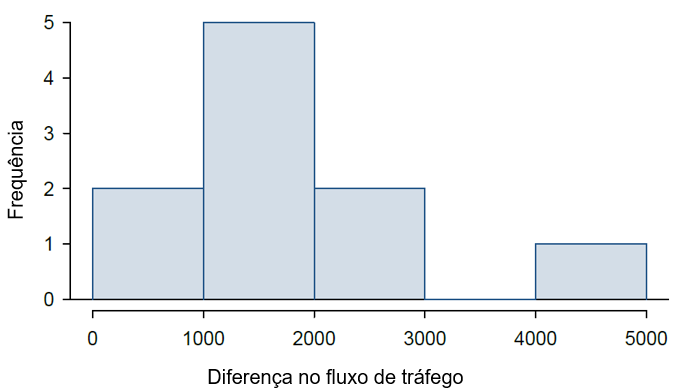
\includegraphics[width=\textwidth]{5-1_one_t/trafficHist.png}
}
\pause
\small
\justifying
\dq{Então, o que fazemos quando o tamanho da amostra é pequeno?}
\end{itemize}

$\:$ \\

\end{frame}

%%%%%%%%%%%%%%%%%%%%%%%%%%%%%%%%%%%

\begin{frame}
\frametitle{Revisão: para que serve um tamanho de amostra grande?}
\justifying
Enquanto as observações forem independentes e a distribuição da população não for extremamente assimétrica, uma grande amostra irá garantir que ...

\begin{itemize}
\justifying
\item a distribuição amostral da média é quase normal
\justifying
\item a estimativa do erro padrão, como $\frac{s}{\sqrt{n}}$, é confiável

\end{itemize}

\end{frame}

%%%%%%%%%%%%%%%%%%%%%%%%%%%%%%%%%%%

\subsection{A condição de normalidade}

%%%%%%%%%%%%%%%%%%%%%%%%%%%%%%%%%%%

\begin{frame}
\frametitle{A condição de normalidade}

\begin{itemize}
\justifying
\item O TCL, que afirma que as distribuições da amostra serão quase normais, vale para \orange{qualquer} tamanho da amostra, desde que a distribuição da população seja quase normal.

\pause
\justifying
\item Embora esse seja um caso especial bastante útil, é inerentemente difícil verificar a normalidade em conjuntos de dados pequenos.

\pause
\justifying
\item Devemos ter cautela ao verificar a condição de normalidade para amostras pequenas. É importante não só examinar os dados, mas também pensar sobre a origem dos dados.
\begin{itemize}
\justifying
\item Por exemplo, se pergunte: eu esperaria que essa distribuição fosse simétrica e estou confiante de que os outliers são raros?
\end{itemize}

\end{itemize}

\end{frame}

%%%%%%%%%%%%%%%%%%%%%%%%%%%%%%%%%%%

\subsection{Apresentando a distribuição $ t $}

%%%%%%%%%%%%%%%%%%%%%%%%%%%%%%%%%%%

\begin{frame}
\frametitle{A distribuição $ t $}

\begin{itemize}
\justifying
\item Quando o desvio padrão da população é desconhecido (o que quase sempre ocorre), a incerteza da estimativa do erro padrão é resolvida usando uma nova distribuição: a \hl{distribuição $ t $}.

\pause
\justifying
\item Essa distribuição também tem formato de sino, mas suas caudas são \hl{mais pesadas} do que as do modelo normal.

\pause
\justifying
\item Portanto, é mais provável que as observações caiam além de dois SDs da média do que sob a distribuição normal.

\pause
\justifying
\item Essas caudas mais pesadas são úteis para resolver nosso problema com uma estimativa menos confiável do erro padrão (já que $n$ é pequeno).

\end{itemize}

\begin{center}
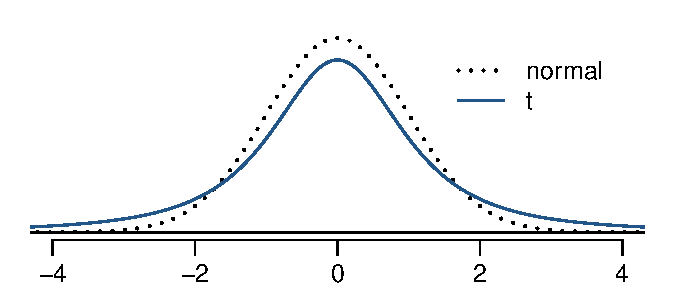
\includegraphics[width=0.4\textwidth]{5-1_one_t/tDistCompareToNormalDist.pdf}
\end{center}

\end{frame}

%%%%%%%%%%%%%%%%%%%%%%%%%%%%%%%%%%%

\begin{frame}
\frametitle{A distribuição $ t $ (cont.)}

\begin{itemize}
\justifying
\item Sempre centralizado em zero, como a distribuição normal padrão ($ z $).
\justifying
\item Tem um único parâmetro \hl{graus de liberdade}: (\mathhl{df}).

\end{itemize}

\begin{center}
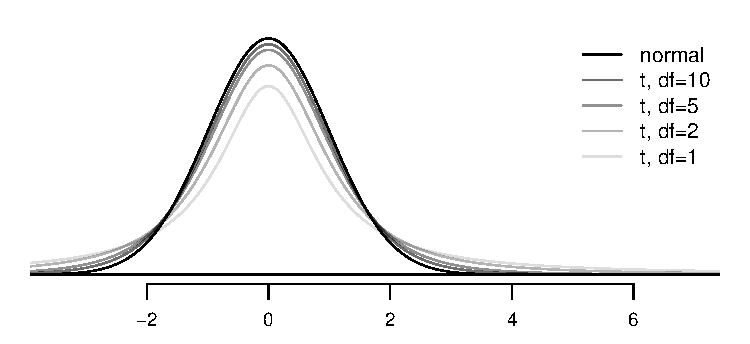
\includegraphics[width=0.8\textwidth]{5-1_one_t/tDistConvergeToNormalDist.pdf}
\end{center}

\pause
\justifying
\dq{O que acontece com a forma da distribuição $t$ quando $df$ aumenta?}
\justifying
\soln{\pause Aproxima-se da normal.}

\end{frame}

%%%%%%%%%%%%%%%%%%%%%%%%%%%%%%%%%%%

\subsection{Avaliando hipóteses usando a distribuição $t$}

%%%%%%%%%%%%%%%%%%%%%%%%%%%%%%%%%%%

\begin{frame}
\frametitle{De volta à sexta-feira 13}

{\scriptsize
\texttt{
\begin{center}
\begin{tabular}{rllrr || r || l}
  \hline
 & tipo & data & dia 6 & dia 13 & qtde & localização  \\ 
  \hline
1 & trafégo & 1990,  Julho & 139246 & 138548 & 698 & loc 1 \\
  \rowcolor[gray]{.9}
  2 & trafégo & 1990,  Julho & 134012 & 132908 & 1104 & loc 2 \\
  3 & trafégo & 1991,  Setembro & 137055 & 136018 & 1037 & loc 1 \\
  \rowcolor[gray]{.9}
  4 & trafégo & 1991,  Setembro & 133732 & 131843 & 1889 & loc 2 \\
  5 & trafégo & 1991,  Dezembro & 123552 & 121641 & 1911 & loc 1 \\
  \rowcolor[gray]{.9}
  6 & trafégo & 1991,  Dezembro & 121139 & 118723 & 2416 & loc 2 \\
  7 & trafégo & 1992,  Março & 128293 & 125532 & 2761 & loc 1 \\
  \rowcolor[gray]{.9}
  8 & trafégo & 1992,  Março & 124631 & 120249 & 4382 & loc 2 \\
  9 & trafégo & 1992,  Novembro & 124609 & 122770 & 1839 & loc 1 \\
  \rowcolor[gray]{.9}
  10 & trafégo & 1992,  Novembro & 117584 & 117263 & 321 & loc 2 \\
   \hline
\end{tabular}
\end{center}
}}
\scriptsize{
\hspace{8cm}\orange{$\downarrow$}
\begin{align*}
\hspace{6cm} &\orange{$\bar{x}_{qtde} = 1836$} \\
& \orange{$s_{qtde} = 1176$} \\
& \orange{$n = 10$} 
\end{align*}
 }
\end{frame}

%%%%%%%%%%%%%%%%%%%%%%%%%%%%%%%%%%%

\begin{frame}
\frametitle{Encontrando a estatística de teste}
\justifying
\formula{Teste estatístico: inferência para média em uma amostra pequena}
{A estatística de teste para inferência sobre a média em uma amostra pequena ($ n <50 $) é a estatística $T$ com $df = n - 1$.
\[ T_{df} = \frac{\text{esmativa pontual} - \text{valor da hipótese nula}}{SE} \]}

\pause

\vspace{-0.5cm}
\justifying
\hl{Neste contexto...}
\begin{eqnarray*}
estimativa~pontual &=& \bar{x}_{qtde} = 1836 \\
\pause
SE &=& \frac{s_{qtde}}{\sqrt{n}} = \frac{1176}{\sqrt{10}} = 372 \\
\pause
T &=& \frac{1836 - 0}{372} = 4.94 \\
\pause
df &=& 10 - 1 = 9
\end{eqnarray*}
\justifying
\scriptsize
\Note{O valor da hipótese nula é 0 porque definimos $\mu_{qtde} = 0$.}

\end{frame}

%%%%%%%%%%%%%%%%%%%%%%%%%%%%%%%%%%%

\begin{frame}[fragile]
\frametitle{Encontrando o valor p}

\begin{itemize}
\justifying
\item O valor p é, mais uma vez, calculado como sendo a área de cauda sob a distribuição $t$.

\pause

\item Usando R:
\begin{verbatim}
> 2 * pt(4.94, df = 9, lower.tail = FALSE)

[1] 0.0008022394
\end{verbatim}

\pause
\justifying
\item Usando a web app:
\justifying
\href{https://gallery.shinyapps.io/dist_calc/}{\textcolor{oiB}{https://gallery.shinyapps.io/dist\_calc/}}

\pause
\justifying
\item Se o app não estiver disponível, podemos usar uma \webLink{https://www.openintro.org/download.php?file=os2_prob_tables&referrer=/stat/textbook.php}{tabela $t$}.

\end{itemize}

\end{frame}

%%%%%%%%%%%%%%%%%%%%%%%%%%%%%%%%%%%

\begin{frame}
\frametitle{Encontrando o valor p}
\justifying
\scriptsize
Localize a estatística $ T $ calculada na linha $ df $ apropriada, obtenha o valor p do cabeçalho da coluna correspondente (uma ou duas linhas, dependendo da hipótese alternativa).

{\scriptsize
\begin{center}
\begin{tabular}{r | rrr rr}
one tail & \hspace{1.5mm}  0.100 & \hspace{1.5mm} 0.050 & \hspace{1.5mm} 0.025 & \hspace{1.5mm} 0.010 & \hspace{1.5mm} 0.005  \\
two tails & 0.200 & 0.100 & 0.050 & 0.020 & 0.010 \\
\hline
{$df$} \hfill 1  &  {  3.08} & {  6.31} & { 12.71} & { 31.82} & { 63.66}  \\ 
2  &  {  1.89} & {  2.92} & {  4.30} & {  6.96} & {  9.92}  \\ 
3  &  {  1.64} & {  2.35} & {  3.18} & {  4.54} & {  5.84}  \\ 
$\vdots$ & $\vdots$ &$\vdots$ &$\vdots$ &$\vdots$ & \\
17  &  {  1.33} & {  1.74} & {  2.11} & {  2.57} & {  2.90}  \\ 
18  &  {  1.33} & {  1.73} & {  2.10} & {  2.55} & {  2.88}  \\ 
19  &  {  1.33} & {  1.73} & {  2.09} & {  2.54} & {  2.86}  \\ 
20  &  {  1.33} & {  1.72} & {  2.09} & {  2.53} & {  2.85}  \\ 
$\vdots$ & $\vdots$ &$\vdots$ &$\vdots$ &$\vdots$ & \\
400  &  {  1.28} & {  1.65} & {  1.97} & {  2.34} & {  2.59}  \\ 
500  &  {  1.28} & {  1.65} & {  1.96} & {  2.33} & {  2.59}  \\ 
$\infty$  &  {  1.28} & {  1.64} & {  1.96} & {  2.33} & {  2.58}  \\ 
\end{tabular}
\end{center}
}
\end{frame}


\begin{frame}
\frametitle{Encontrando o valor p (cont.)}


{\scriptsize
\begin{center}
\begin{tabular}{r | rrr rr}
\hline
one tail & \hspace{1.5mm}  0.100 & \hspace{1.5mm} 0.050 & \hspace{1.5mm} 0.025 & \hspace{1.5mm} 0.010 & \hspace{1.5mm} 0.005  \\
two tails & 0.200 & 0.100 & 0.050 & 0.020 & 0.010 \\
\hline
{df} \hfill 6  &  {  1.44} & {  1.94} & {  2.45} & {  3.14} & {  3.71}  \\ 
7  &  {  1.41} & {  1.89} & {  2.36} & {  3.00} & {  3.50}  \\ 
8  &  {  1.40} & {  1.86} & {  2.31} & {  2.90} & {  3.36}  \\ 
  \rowcolor[gray]{.6}
9  &  {  1.38} & {  1.83} & {  2.26} & {  2.82} & {  3.25}  \\ 
10  &  {  1.37} & {  1.81} & {  2.23} & {  2.76} & {  3.17}  \\ 
\end{tabular}
\vspace{1cm}
\twocol{0.5}{0.5}{
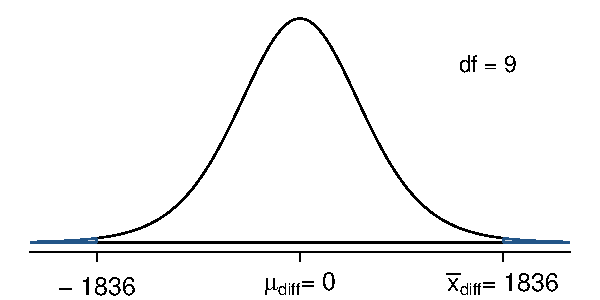
\includegraphics[width=1.1\textwidth]{5-1_one_t/fridayPvalue.pdf}
}
{
$T = 4.94$}

\end{center}
}

\end{frame}

%%%%%%%%%%%%%%%%%%%%%%%%%%%%%%%%%%%

\begin{frame}
\frametitle{Conclusão do teste}
\justifying
\dq{Qual é a conclusão do teste de hipóteses?}
\justifying
\pause
\soln{Os dados fornecem evidências convincentes de uma diferença entre o fluxo de tráfego na sexta-feira 6 e 13.}


\end{frame}

%%%%%%%%%%%%%%%%%%%%%%%%%%%%%%%%%%%%

\subsection{Construindo intervalos de confiança usando a distribuição $t$}

%%%%%%%%%%%%%%%%%%%%%%%%%%%%%%%%%%%

\begin{frame}
\frametitle{Qual é a diferença?}

\begin{itemize}
\justifying
\item Concluímos que há uma diferença no fluxo de tráfego entre sexta-feira 6 e 13.

\pause
\justifying
\item Mas seria mais interessante descobrir exatamente que diferença é essa.

\pause
\justifying
\item Podemos usar um intervalo de confiança para estimar essa diferença.

\end{itemize}

\end{frame}

%%%%%%%%%%%%%%%%%%%%%%%%%%%%%%%%%%%

\begin{frame}
\frametitle{Intervalo de confiança para uma média em uma amostra pequena}

\begin{itemize}
\justifying
\item Os intervalos de confiança são sempre da forma
\[ \text{estimativa pontual} \pm {ME} \]

\pause
\justifying
\item ME é sempre calculado como o produto entre o valor crítico e o SE.

\pause
\justifying
\item Uma vez que uma amostra pequena significa uma distribuição de $t$ (e não uma distribuição de $z$), o valor crítico é $t^{\star}$ (ao contrário de $z^{\star}$).
\[ \text{estimativa pontual} \pm t^{\star} \times SE \]

\end{itemize}

\end{frame}

%%%%%%%%%%%%%%%%%%%%%%%%%%%%%%%%%%%

\begin{frame}
\frametitle{Encontrando o valor crítico $t$ ($t^\star$)}

\twocol{0.5}{0.5}{
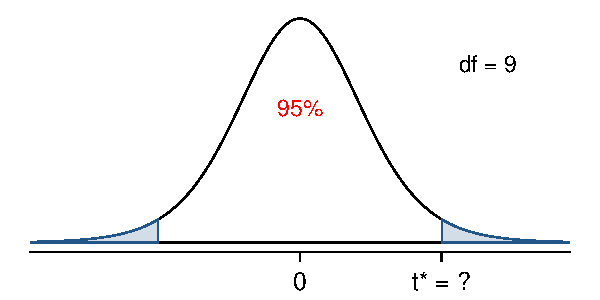
\includegraphics[width=\textwidth]{5-1_one_t/middle95_1.pdf}
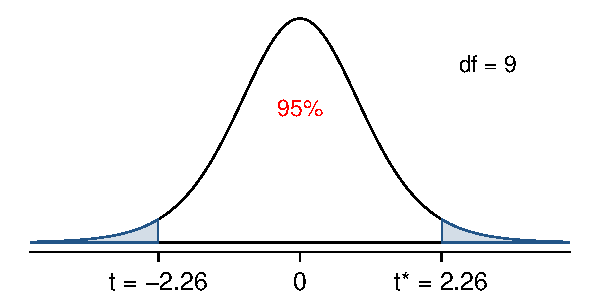
\includegraphics[width=\textwidth]{5-1_one_t/middle95_2.pdf}
}
{\justifying
$n = 10$, $df = 10 - 1 = 9$, $t^\star$ está na interseção da linha $ df = 9 $ e duas probabilidades da cauda 0.05.
}

\end{frame}
%%%%%%%%%%%%%%%%%%%%%%%%%%%%%%%%%%%

\begin{frame}
\frametitle{Encontrando o crítico $t$ ($t^\star$)}
\only<1>{
{\small
\begin{center}
\begin{tabular}{r | r r r r r}
\hline
Uma cauda & \hspace{1.5mm}  0.100 & \hspace{1.5mm} 0.050 & \hspace{1.5mm} 0.025 & \hspace{1.5mm} 0.010 & \hspace{1.5mm} 0.005  \\
duas caudas & 0.200 & 0.100 & 0.050 & 0.020 & {0.010} \\
\hline
{df} \hfill 6  &  {  1.44} & {  1.94} & {  2.45} & {  3.14} & {  3.71}  \\ 
7  &  {  1.41} & {  1.89} & {  2.36} & {  3.00} & {  3.50}  \\ 
8  &  {  1.40} & {  1.86} & {  2.31} & {  2.90} & {  3.36}  \\ 
9  &  {  1.38} & {  1.83} & {  2.26} & {  2.82} & {  3.25} \\ 
10  &  {  1.37} & {  1.81} & {  2.23} & {  2.76} & {  3.17}  \\ 
\end{tabular}
\end{center}
}}

\only<2 | handout:0>{
{\small
\begin{center}
\begin{tabular}{r | r r r r r}
\hline
Uma cauda & \hspace{1.5mm}  0.100 & \hspace{1.5mm} 0.050 & \hspace{1.5mm} 0.025 & \hspace{1.5mm} 0.010 & \hspace{1.5mm} 0.005  \\
duas caudas & 0.200 & 0.100 & 0.050 & 0.020 & {0.010} \\
\hline
{df} \hfill 6  &  {  1.44} & {  1.94} & {  2.45} & {  3.14} & {  3.71}  \\ 
7  &  {  1.41} & {  1.89} & {  2.36} & {  3.00} & {  3.50}  \\ 
8  &  {  1.40} & {  1.86} & {  2.31} & {  2.90} & {  3.36}  \\ 
  \rowcolor[gray]{.6}
9  &  {  1.38} & {  1.83} & {  2.26} & {  2.82} & {  3.25} \\ 
10  &  {  1.37} & {  1.81} & {  2.23} & {  2.76} & {  3.17}  \\ 
\end{tabular}
\end{center}
}}

\only<3 | handout:0>{
{\small
\begin{center}
\begin{tabular}{r | r r >{\columncolor[gray]{.6}[.5\tabcolsep]}r r r}
\hline
Uma cauda & \hspace{1.5mm}  0.100 & \hspace{1.5mm} 0.050 & \hspace{1.5mm} 0.025 & \hspace{1.5mm} 0.010 & \hspace{1.5mm} 0.005  \\
duas caudas & 0.200 & 0.100 & \orange{0.050} & 0.020 & {0.010} \\
\hline
{df} \hfill 6  &  {  1.44} & {  1.94} & {  2.45} & {  3.14} & {  3.71}  \\ 
7  &  {  1.41} & {  1.89} & {  2.36} & {  3.00} & {  3.50}  \\ 
8  &  {  1.40} & {  1.86} & {  2.31} & {  2.90} & {  3.36}  \\ 
  \rowcolor[gray]{.6}
9  &  {  1.38} & {  1.83} & {  2.26} & {  2.82} & {  3.25} \\ 
10  &  {  1.37} & {  1.81} & {  2.23} & {  2.76} & {  3.17}  \\ 
\end{tabular}
\end{center}
}}

\only<4 | handout:0>{
{\small
\begin{center}
\begin{tabular}{r | r r >{\columncolor[gray]{.6}[.5\tabcolsep]}r r r}
\hline
Uma cauda & \hspace{1.5mm}  0.100 & \hspace{1.5mm} 0.050 & \hspace{1.5mm} 0.025 & \hspace{1.5mm} 0.010 & \hspace{1.5mm} 0.005  \\
duas caudas & 0.200 & 0.100 & \orange{0.050} & 0.020 & {0.010} \\
\hline
{df} \hfill 6  &  {  1.44} & {  1.94} & {  2.45} & {  3.14} & {  3.71}  \\ 
7  &  {  1.41} & {  1.89} & {  2.36} & {  3.00} & {  3.50}  \\ 
8  &  {  1.40} & {  1.86} & {  2.31} & {  2.90} & {  3.36}  \\ 
  \rowcolor[gray]{.6}
9  &  {  1.38} & {  1.83} & \orange{  2.26} & {  2.82} & {  3.25} \\ 
10  &  {  1.37} & {  1.81} & {  2.23} & {  2.76} & {  3.17}  \\ 
\end{tabular}
\end{center}
}}


\end{frame}

%%%%%%%%%%%%%%%%%%%%%%%%%%%%%%%%%%%

\begin{frame}
\frametitle{Construindo um IC para uma média pequena de amostra}
\justifying
\pq{Qual dos seguintes é o cálculo correto de um intervalo de confiança de 95\% para a diferença entre o fluxo de tráfego entre sexta-feira 6 e 13?}
\[ \bar{x}_{qtde} = 1836 \qquad s_{qtde} = 1176 \qquad n = 10 \qquad SE = 372 \]

\twocol{0.35}{0.65}
{
\begin{enumerate}[(a)]

\item $1836 \pm 1.96 \times 372$

\solnMult{ $1836 \pm 2.26 \times 372$}

\item $1836 \pm -2.26 \times 372$

\item $1836 \pm 2.26 \times 1176$

\end{enumerate}
}
{
\soln{\only<2>{\orange{$\rightarrow$ (995, 2677)}}}
\vspace{0.25cm}
}

\end{frame}

%%%%%%%%%%%%%%%%%%%%%%%%%%%%%%%%%%%

\begin{frame}
\frametitle{Interpretando o IC}
\justifying
\pq{Qual das seguintes opções é a \orange{melhor} interpretação para o intervalo de confiança que acabamos de calcular?
\[ \mu_{qtde: 6 - 13} = (995, 2677) \]
}
\justifying
Estamos 95\% confiantes de que ...

\begin{enumerate}[(a)]
\justifying
\item a diferença entre o número médio de carros na estrada na sexta-feira 6 e 13 é entre 995 e 2.677.
\justifying
\item na sexta-feira 6 há 995 a 2.677 carros a menos na estrada do que na sexta-feira 13, em média.
\justifying
\item na sexta-feira 6 há, em média, 995 carros a menos e na sexta-feira 13 há, em média, 2.677 carros a mais na estrada.
\justifying
\solnMult{na sexta-feira 13 há de 995 a 2.677 carros a menos na estrada do que na sexta-feira 6, em média.}

\end{enumerate}

\end{frame}

%%%%%%%%%%%%%%%%%%%%%%%%%%%%%%%%%%%

\subsection{Síntese}

%%%%%%%%%%%%%%%%%%%%%%%%%%%%%%%%%%%

\begin{frame}
\frametitle{Síntese}
\justifying
\dq{A conclusão do teste de hipótese concorda com o que encontramos para o intervalo de confiança?}

$\:$ \\
\justifying
\soln{\only<2->{Sim, o teste de hipótese encontrou uma diferença significativa e o IC não contém o valor da hipótese nula que é igual zero.}}

$\:$ \\
\justifying
\dq{Você acha que as descobertas deste estudo sugerem que as pessoas acreditam que sexta-feira 13 é um dia de má sorte?}

$\:$ \\
\justifying
\soln{\only<3>{Não, este é um estudo observacional. Acabamos de observar uma diferença significativa entre o número de carros na estrada nesses dois dias. Nós não testamos as crenças das pessoas.}}

\end{frame}

%%%%%%%%%%%%%%%%%%%%%%%%%%%%%%%%%%%

\begin{frame}

\frametitle{Recapitulando: Inferência usando a distribuição $t$}

\begin{itemize}

\justifying
\item Se $ \sigma $ for desconhecido, use a distribuição $t$ com $SE = \frac{s}{\sqrt {n}}$.

\pause
\justifying
\item Condições: 
\begin{itemize}
\justifying
\item independência das observações (usar amostragem aleatória, e se a amostragem for sem reposição, $n <$ 10\% da população)
\justifying
\item nenhum desvio extremo
\end{itemize}

\end{itemize}

\end{frame}

\begin{frame}

\frametitle{Recapitulando: Inferência usando a distribuição $t$}

\begin{itemize}
\justifying

\item Teste de hipóteses: 
\[ T_{df} = \frac{\text{estimativa pontual} - \text{valor da hipótese nula}}{SE}\text{, onde }df = n - 1 \]

\pause
\justifying
\item Intervalo de confiança:
\[ \text{estimativa pontual} \pm t_{df}^\star \times SE \]

\end{itemize}

\pause
\Note{\scriptsize O exemplo que usamos foi para médias pareadas (diferença entre grupos dependentes). Tomamos a diferença entre as observações e usamos apenas essas diferenças (uma amostra) em nossa análise, portanto, a mecânica é a mesma de quando estamos trabalhando com apenas uma amostra.}
\end{frame}

%%%%%%%%%%%%%%%%%%%%%%%%%%%%%%%%%%%%

\section{5.2. Dados pareados}

%%%%%%%%%%%%%%%%%%%%%%%%%%%%%%%%%%%

\subsection{Observações pareados}

\begin{frame}
\frametitle{Prática}
\justifying
\dq{Foram amostradas aleatoriamente 200 observações em uma pesquisa na High School and Beyond. Os alunos fizeram um teste de leitura e escrita. À primeira vista, parece haver uma diferença entre a pontuação média do teste de leitura e escrita?}

\begin{center}
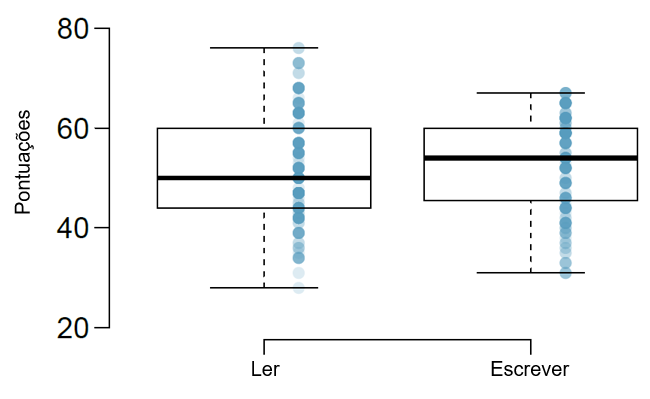
\includegraphics[width=0.5\textwidth]{5-2_paired/hsb2_read_write_box.png}
\end{center}

\end{frame}

%%%%%%%%%%%%%%%%%%%%%%%%%%%%%%%%%%%%

\begin{frame}
\frametitle{Prática}
\justifying
\pq{As notas de leitura e escrita de cada aluno são independentes umas das outras?}

{\small
\begin{center}
\begin{tabular}{rrrr}
  \hline
 & id & leitura & escrita \\ 
  \hline
1 & 70 & 57 & 52 \\ 
  2 & 86 & 44 & 33 \\ 
  3 & 141 & 63 & 44 \\ 
  4 & 172 & 47 & 52 \\ 
  $\vdots$ &   $\vdots$  &   $\vdots$ &   $\vdots$  \\
  200 & 137 & 63 & 65 \\ 
   \hline
\end{tabular}
\end{center}
}

\begin{multicols}{2}
\begin{enumerate}[(a)]
\item Sim
\solnMult{Não}
\end{enumerate}
\end{multicols}

\end{frame}

%%%%%%%%%%%%%%%%%%%%%%%%%%%%%%%%%%%%

\begin{frame}
\frametitle{Analisando dados pareados}
\small
\begin{itemize}
\justifying
\item Quando dois conjuntos de observações têm essa correspondência especial (não independente), diz-se que são \hl{pareados}.

\pause
\justifying
\item Para analisar dados pareados, é frequentemente útil observar a diferença nos resultados de cada par de observações. \\

\centering diferenca = leitura - escrita \\

\pause
\justifying
\item É importante subtrairmos sempre usando uma ordem consistente.

\end{itemize}

\pause
\begin{columns}
\begin{column}{0.5\textwidth}
{\scriptsize
\begin{center}
\begin{tabular}{rrrr >{\columncolor[gray]{.9}}r}
 \hline

 & id & leitura & escrita & diferença \\ 
  \hline
1 & 70 & 57 & 52 & 5 \\ 
  2 & 86 & 44 & 33 & 11 \\ 
  3 & 141 & 63 & 44 & 19 \\ 
  4 & 172 & 47 & 52 & -5 \\ 
  $\vdots$ &   $\vdots$  &   $\vdots$ &   $\vdots$ &   $\vdots$ \\
  200 & 137 & 63 & 65 & -2 \\ 
   \hline
\end{tabular}
\end{center}}
\end{column}
\begin{column}{0.5\textwidth}  %%<--- here
    \begin{center}
     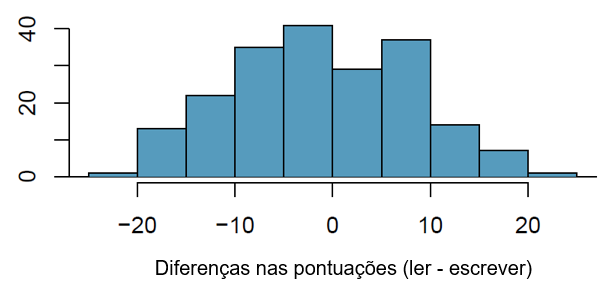
\includegraphics[width=1.15\textwidth]{5-2_paired/hsb2_diff_hist.png}
     \end{center}
\end{column}
\end{columns}

\end{frame}



%%%%%%%%%%%%%%%%%%%%%%%%%%%%%%%%%%%%

\begin{frame}
\frametitle{Estimativa de parâmetro e de ponto}

\begin{itemize}
\justifying
\item \hl{Parâmetro de interesse:} Diferença média entre as pontuações de leitura e escrita de \orange{todos} estudantes do ensino médio.
\[ \mu_{diferenca} \]

$\:$ \\

\pause
\justifying
\item \hl{Estimativa pontual:} Diferença média entre as pontuações de leitura e escrita de estudantes do ensino médio \orange{amostrado}.
\[ \bar{x}_{diferenca} \]

\end{itemize}

\end{frame}

%%%%%%%%%%%%%%%%%%%%%%%%%%%%%%%%%%%%

\subsection{Inferência para dados pareados}

\begin{frame}
\frametitle{Definindo as hipóteses}
\justifying
\dq{Se, de fato, não houve diferença entre as pontuações nos exames de leitura e escrita, como você esperaria que a diferença média fosse?}

\pause

\soln{0}

$\:$ \\

\pause
\justifying
\dq{Quais são as hipóteses para testar se existe uma diferença entre as pontuações médias de leitura e escrita?}

\pause

\begin{itemize}
\justifying
\item[$H_0$:] Não há diferença entre a pontuação média de leitura e escrita.
\[ \mu_{diferenca} = 0 \]
\justifying
\item[$H_A$:] Existe uma diferença entre a pontuação média de leitura e escrita.
\[ \mu_{diferenca} \ne 0 \]
\end{itemize}

\end{frame}

%%%%%%%%%%%%%%%%%%%%%%%%%%%%%%%%%%%%

\begin{frame}
\frametitle{Nada de novo aqui}

\begin{itemize}
\justifying
\item A análise não é diferente do que fizemos antes.
\justifying
\item Temos dados de \orange{uma} amostra: diferenças.
\justifying
\item Estamos testando para ver se a diferença média é diferente de 0.

\end{itemize}

\end{frame}

%%%%%%%%%%%%%%%%%%%%%%%%%%%%%%%%%%%%

\begin{frame}
\frametitle{Verificação de suposições \& condições}
\justifying
\pq{Qual dos seguintes é verdadeiro?}

\begin{enumerate}[(a)]
\justifying
\solnMult{Como os alunos são amostrados aleatoriamente e são menores que 10\% de todos os alunos do ensino médio, podemos supor que a diferença entre os escores de leitura e escrita de um aluno na amostra é independente do outro.}
\justifying
\item A distribuição das diferenças é bimodal, portanto não podemos continuar com o teste de hipóteses.
\justifying
\item Para que as diferenças sejam aleatórias, devemos ter amostras com reposição.
\justifying
\item Como os alunos são amostrados aleatoriamente e são menores que 10\% de todos os alunos, podemos supor que a distribuição amostral da diferença média será quase normal.
\end{enumerate}

\end{frame}

%%%%%%%%%%%%%%%%%%%%%%%%%%%%%%%%%%%

\begin{frame}[shrink]
\frametitle{Calculando a estatística de teste e o valor p}
\justifying
\dq{A diferença média observada entre as duas pontuações é de -0,545 pontos e o desvio padrão da diferença é de 8,887 pontos. Esses dados fornecem evidências convincentes de uma diferença entre as pontuações médias dos dois exames? Usar $\alpha = 0.05$.}

\twocol{0.5}{0.5}
{
\begin{center}
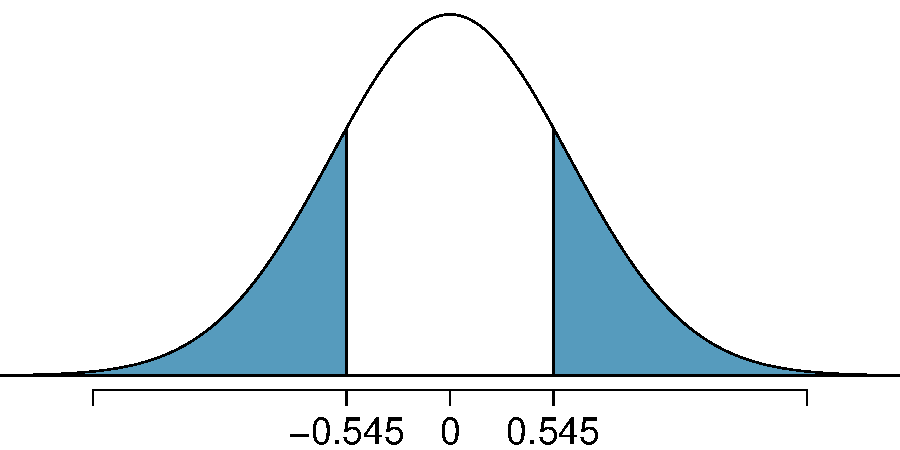
\includegraphics[width=\textwidth]{5-2_paired/hsb2_read_write_pval.pdf}
\end{center}
}
{
\pause
\begin{eqnarray*}
T &=& \frac{-0.545 - 0}{\frac{8.887}{\sqrt{200}}} \\
&=& \frac{-0.545}{0.628} = -0.87 \\
df &=& 200 - 1 = 199 \\
\pause
valor-p &=& 0.1927 \times 2 = 0.3854
\end{eqnarray*}
}
\pause 
$\:$ \\
\justifying
Como o valor de p $> $ 0,05, não é possível rejeitar, os dados \underline {não} fornecem evidências convincentes de uma diferença entre as pontuações médias de leitura e escrita.

\end{frame}

%%%%%%%%%%%%%%%%%%%%%%%%%%%%%%%%%%%

\begin{frame}
\frametitle{Interpretação do valor p}
\justifying
\pq{Qual das seguintes é a interpretação correta do valor p?}

\begin{enumerate}[(a)]
\justifying
\item Probabilidade de que as pontuações médias nos exames de leitura e escrita sejam iguais.
\justifying
\item Probabilidade de que as pontuações médias nos exames de leitura e escrita sejam diferentes.
\justifying
\solnMult{Probabilidade de obter uma amostra aleatória de 200 alunos, onde a diferença média entre as pontuações de leitura e escrita é de pelo menos 0.545 (em qualquer direção), se de fato a diferença média real entre as pontuações é 0.}
\justifying
\item Probabilidade de rejeitar incorretamente a hipótese nula se, de fato, a hipótese nula for verdadeira.
\end{enumerate}

\end{frame}

%%%%%%%%%%%%%%%%%%%%%%%%%%%%%%%%%%%%

\begin{frame}
\frametitle{TH $\leftrightarrow$ IC}
\justifying
\pq{Suponha que fôssemos construir um intervalo de confiança de 95\% para a diferença média entre as pontuações de leitura e escrita. Você esperaria que esse intervalo incluísse 0?}

\begin{enumerate}[(a)]
\justifying
\solnMult{sim}
\justifying
\item não
\justifying
\item não posso dizer a partir da informação dada
\end{enumerate}

\soln{\pause
\begin{eqnarray*} 
-0.545 \pm 1.97 \frac{8.887}{\sqrt{200}} &=& -0.545 \pm 1.97 \times 0.628 \\
&=& -0.545 \pm 1.24 \\
&=& (-1.785, 0.695)
\end{eqnarray*}
}

\end{frame}

%%%%%%%%%%%%%%%%%%%%%%%%%%%%%%%%%%%%


%%%%%%%%%%%%%%%%%%%%%%%%%%%%%%%%%%%%

\section{5.3. Diferença de duas médias}

%%%%%%%%%%%%%%%%%%%%%%%%%%%%%%%%%%%%

\begin{frame}
\frametitle{Diamantes}

\begin{itemize}
\justifying
\item Pesos de diamantes são medidos em quilates. 
\justifying
\item 1 quilate = 100 pontos, 0,99 quilates = 99 pontos, etc.
\justifying
\item A diferença entre o tamanho de um diamante de 0,99 quilates e um diamante de 1 quilate é indetectável a olho nu, mas o preço de um diamante de 1 quilate tende a ser maior do que o preço de um diamante de 0,99 quilates?
\justifying
\item Vamos testar para ver se existe uma diferença entre os preços médios de diamantes de 0,99 e 1 quilates.
\justifying
\item Para podermos comparar unidades equivalentes, dividimos os preços de 0,99 quilates em 99 e de 1 quilate em 100, e comparamos os preços médios em pontos.

\end{itemize}

\hfill 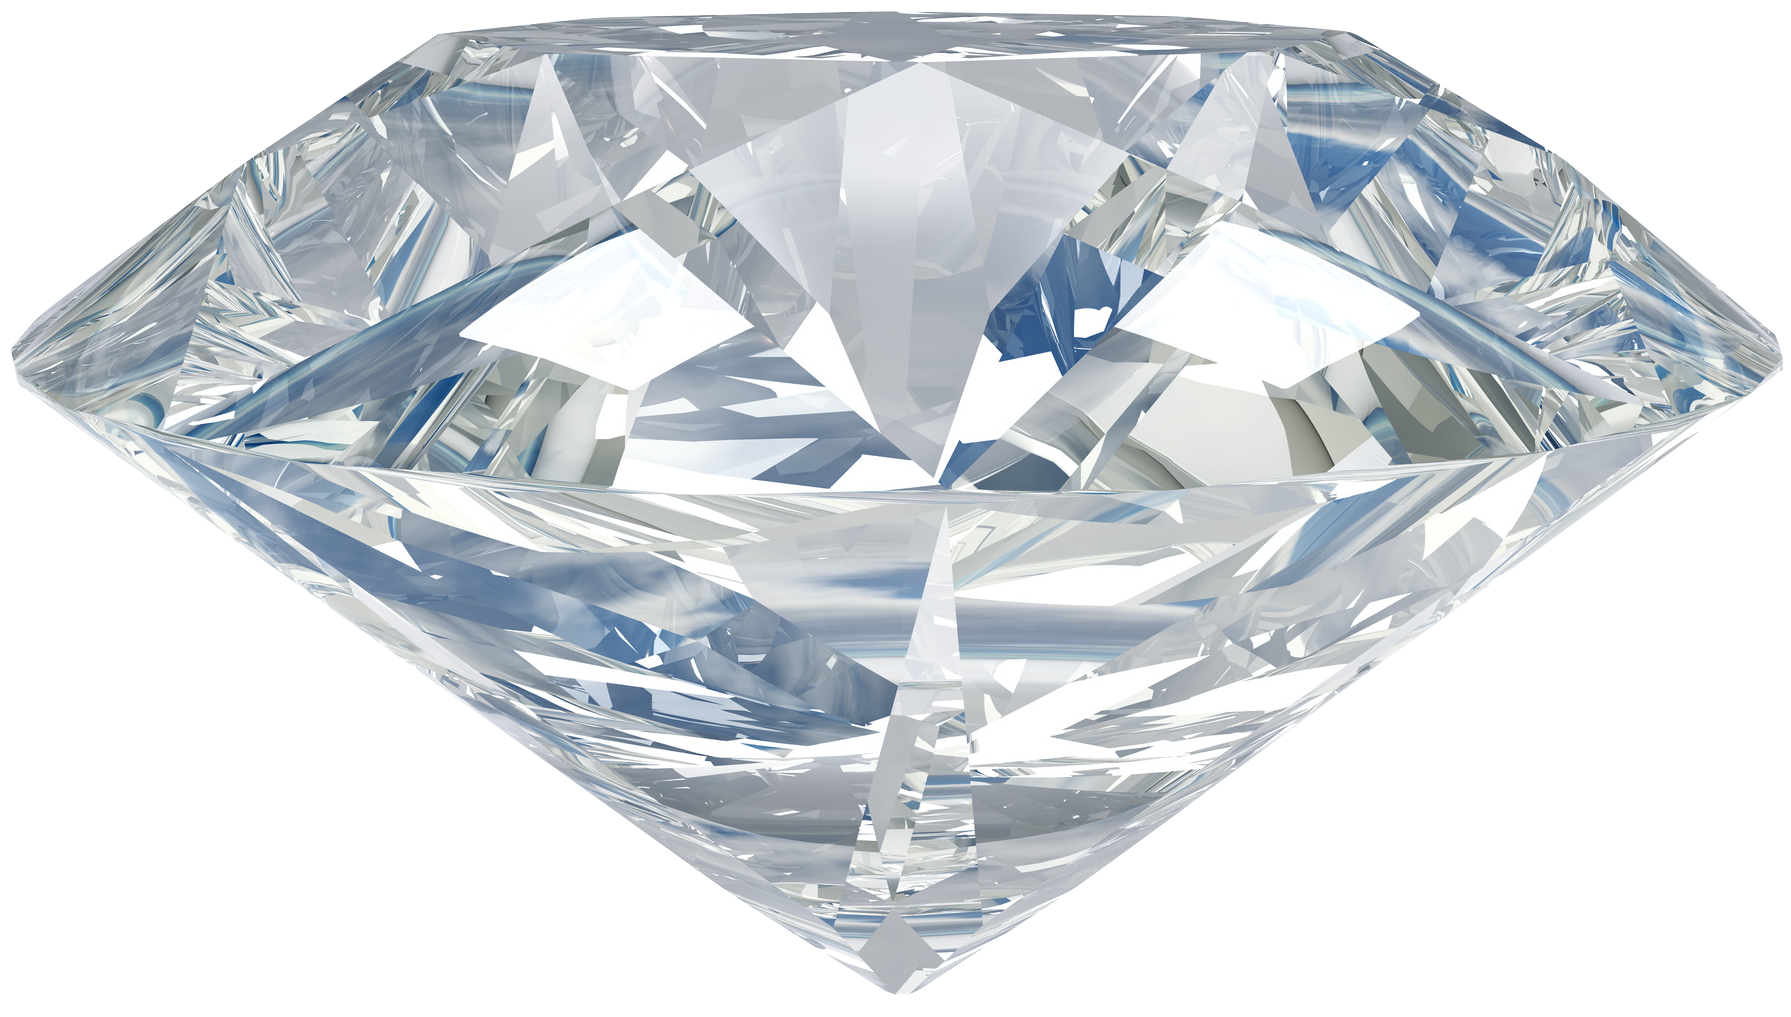
\includegraphics[width=0.2\textwidth]{5-3_diff_two_mean/diamond.png}

\end{frame}

%%%%%%%%%%%%%%%%%%%%%%%%%%%%%%%%%%%

\begin{frame}[fragile]
\frametitle{Dados}

\begin{center}
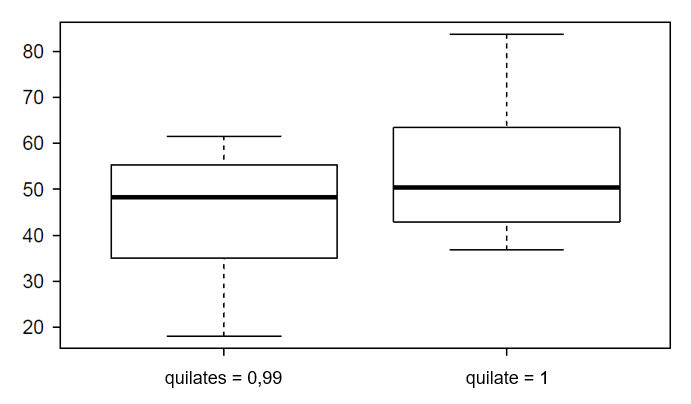
\includegraphics[width=0.6\textwidth]{5-3_diff_two_mean/diamondBox.png}
\end{center}

{\small
\begin{center}
\begin{tabular}{l | c | c}
		& {\footnotesize \hl{0.99 quilate}} &  {\footnotesize \hl{1 quilate}}  \\
		& pt99	& pt100 \\
\hline
$\bar{x}$	& 44.50		& 53.43 \\
$s$		& 13.32		& 12.22 \\
$n$		& 23			& 30
\end{tabular}
\end{center}
}

\vfill

\rule{2.5cm}{0.25pt} \\
\justifying
{\tiny Estes dados são uma amostra aleatória do conjunto de dados \texttt {diamonds} no pacote do R \texttt {ggplot2}.}

\end{frame}

%%%%%%%%%%%%%%%%%%%%%%%%%%%%%%%%%%%

\begin{frame}
\frametitle{Estimativa de parâmetro e ponto}

\begin{itemize}
\justifying
\item \hl{Parâmetro de interesse:} Diferença média entre os preços em pontos de \orange{todos} os diamantes de 0,99 quilates e de 1 quilate.
\[ \mu_{pt99} - \mu_{pt100} \]

$\:$ \\

\pause
\justifying
\item \hl{Estimativa pontual:} Diferença média entre os preços em pontos da \orange{amostra} de diamantes de 0,99 quilates e 1 quilate.
\[ \bar{x}_{pt99} - \bar{x}_{pt100} \]

\end{itemize}

\end{frame}

%%%%%%%%%%%%%%%%%%%%%%%%%%%%%%%%%%%

\begin{frame}
\frametitle{Hipótese}
\justifying
\pq{Qual das alternativas a seguir é o conjunto correto de hipóteses para testar se o preço médio dos diamantes de 1 quilate ($ _{pt100} $) é maior que o preço médio dos diamantes de 0,99 quilates ($_{pt99}$)?}

\begin{enumerate}[(a)]

\item  \mathhl{H_0:} $\mu_{pt99} = \mu_{pt100}$ \\
\mathhl{H_A:} $\mu_{pt99} \ne \mu_{pt100}$

\item  \mathhl{H_0:} $\mu_{pt99} = \mu_{pt100}$ \\
\mathhl{H_A:} $\mu_{pt99} > \mu_{pt100}$

\solnMult{  \mathhl{H_0:} $\mu_{pt99} = \mu_{pt100}$ \\
\mathhl{H_A:} $\mu_{pt99} < \mu_{pt100}$ }

\item  \mathhl{H_0:} $\bar{x}_{pt99} = \bar{x}_{pt100}$ \\
\mathhl{H_A:} $\bar{x}_{pt99} < \bar{x}_{pt100}$

\end{enumerate}

\end{frame}

%%%%%%%%%%%%%%%%%%%%%%%%%%%%%%%%%%%

\begin{frame}
\frametitle{Condições}
\justifying
\pq{Qual dos seguintes itens \underline{não} precisa ser satisfeito para conduzir este teste de hipótese usando métodos teóricos?}

\begin{enumerate}[(a)]
\justifying
\item O preço do ponto de um diamante de 0,99 quilates na amostra deve ser independente do outro, e o preço em pontos de um diamante de 1 quilate deve ser independente do outro.
\justifying
\item Os preços pontuais de 0,99 quilates e 1 quilate de diamantes na amostra devem ser independentes.
\justifying
\item Distribuições de preços pontuais de 0,99 e 1 quilate de diamantes não devem ser extremamente assimétrico.
\justifying
\solnMult{Ambos os tamanhos de amostra devem ser pelo menos 30.}

\end{enumerate}

\end{frame}

%%%%%%%%%%%%%%%%%%%%%%%%%%%%%%%%%%%%

\subsection{Distribuição amostral para a diferença de duas médias}

%%%%%%%%%%%%%%%%%%%%%%%%%%%%%%%%%%%%

\begin{frame}
\frametitle{Estatística de teste}
\justifying
\formula{Teste estatístico para inferência sobre a diferença de duas médias amostrais pequenas}
\justifying
{A estatística de teste para inferência sobre a diferença de duas médias onde $\sigma_1$ e $\sigma_2$ são desconhecidos é a estatística $T$.
\vspace{0.3 cm}
\[ T_{df} = \frac{\text{estimativa pontual} - \text{valor da hipótese nula}}{SE} \]
onde 
\[ SE = \sqrt{ \frac{s_1^2}{n_1} + \frac{s_2^2}{n_2} } \qquad \text{ e } \qquad df = min(n_1 - 1, n_2 - 1) \]
}\justifying
\justifying
\Note{O cálculo do $df$ é realmente muito mais complicado. Para simplificar, usaremos a fórmula acima para \underline{estimar} o verdadeiro $df$ ao conduzir a análise à mão.}

\end{frame}

%%%%%%%%%%%%%%%%%%%%%%%%%%%%%%%%%%%%

\subsection{Teste de hipóteses para a diferença de duas médias}

%%%%%%%%%%%%%%%%%%%%%%%%%%%%%%%%%%%%

\begin{frame}
\frametitle{Estatística de teste (cont.)}

{\small
\begin{center}
\begin{tabular}{l | c | c}
		& {\footnotesize \hl{0.99 quilate}} &  {\footnotesize \hl{1 quilate}}  \\
		& pt99	& pt100 \\
\hline
$\bar{x}$	& 44.50		& 53.43 \\
$s$		& 13.32		& 12.22 \\
$n$		& 23			& 30
\end{tabular}
\end{center}
}

\hl{Neste contexto...}

\pause

{\small
\begin{eqnarray*}
T &=& \frac{\text{estimativa pontual} - \text{valor da hipótese nula} }{SE} \\
\pause
&=& \frac{(44.50 - 53.43) - 0}{ \sqrt{\frac{13.32^2}{23} + \frac{12.22^2}{30} }} \\
\pause
&=& \frac{-8.93}{3.56} \\
\pause
&=& -2.508
\end{eqnarray*}
}

\end{frame}

%%%%%%%%%%%%%%%%%%%%%%%%%%%%%%%%%%%%

\begin{frame}
\frametitle{Estatística de teste (cont.)}
\justifying
\pq{Qual dos seguintes é o $df$ correto para este teste de hipótese?}

\twocol{0.3}{0.7}
{
\begin{enumerate}[(a)]
\solnMult{ 22 }
\item 23
\item 30
\item 29
\item 52
\end{enumerate}
}
{
\soln{\only<2>{
\orange{$\rightarrow df = min(n_{pt99} - 1, n_{pt100} - 1)$ \\
$= min(23 - 1, 30 - 1)$ \\
$= min(22,29) = 22$} \\
\vspace{1cm}
}}}

\end{frame}

%%%%%%%%%%%%%%%%%%%%%%%%%%%%%%%%%%%%

\begin{frame}
\frametitle{valor-p}
\justifying
\pq{Qual dos seguintes é o valor p correto para este teste de hipótese?}

\[ T = -2.508 \qquad \only<1-2 | handout:0>{df = 22} \] 

\twocol{0.42}{0.58}
{
\begin{enumerate}[(a)]
\item entre 0.005 e 0.01
\solnMult{entre 0.01 e 0.025}
\item entre 0.02 e 0.05
\item entre 0.01 e 0.02
\end{enumerate}
}
{
\only<1>{
{
\scalefont{0.47}
\begin{tabular}{r | r r  r r r}
\hline
uma cauda & \hspace{1.5mm}  0.100 & \hspace{1.5mm} 0.050 & \hspace{1.5mm} {0.025} & \hspace{1.5mm} {0.010} & \hspace{1.5mm} 0.005  \\
duas caudas & 0.200 & 0.100 & 0.050 & 0.020 & 0.010 \\
\hline
df \hfill 21  &  {  1.32} & {  1.72} & {  2.08} & {  2.52} & {  2.83}  \\ 
22  &  {  1.32} & {  1.72} & {  2.07} & {  2.51} & {  2.82}  \\ 
23  &  {  1.32} & {  1.71} & {  2.07} & {  2.50} & {  2.81}  \\ 
24  &  {  1.32} & {  1.71} & {  2.06} & {  2.49} & {  2.80}  \\ 
25  &  {  1.32} & {  1.71} & {  2.06} & {  2.49} & {  2.79}  \\ 
\hline
\end{tabular}
}
}

\only<2|handout:0>{
{\scalefont{0.47}
\begin{tabular}{r | r r  >{\columncolor[gray]{.6}[.5\tabcolsep]}r  >{\columncolor[gray]{.6}[.5\tabcolsep]}r r}
\hline
uma cauda & \hspace{1.5mm}  0.100 & \hspace{1.5mm} 0.050 & \hspace{1.5mm} \orange{0.025} & \hspace{1.5mm} \orange{0.010} & \hspace{1.5mm} 0.005  \\
duas caudas & 0.200 & 0.100 & 0.050 & 0.020 & 0.010 \\
\hline
df \hfill 21  &  {  1.32} & {  1.72} & {  2.08} & {  2.52} & {  2.83}  \\ 
  \rowcolor[gray]{.6}
22  &  {  1.32} & {  1.72} & \orange{  2.07} & \orange{  2.51} & {  2.82}  \\ 
23  &  {  1.32} & {  1.71} & {  2.07} & {  2.50} & {  2.81}  \\ 
24  &  {  1.32} & {  1.71} & {  2.06} & {  2.49} & {  2.80}  \\ 
25  &  {  1.32} & {  1.71} & {  2.06} & {  2.49} & {  2.79}  \\ 
\hline
\end{tabular}
}
}}

\end{frame}

%%%%%%%%%%%%%%%%%%%%%%%%%%%%%%%%%%%%

\begin{frame}
\frametitle{Síntese}
\justifying
\dq{Qual é a conclusão do teste de hipóteses? Como essa conclusão mudaria seu comportamento se você comprasse diamantes?}


\soln{\only<2>{
\begin{itemize}
\justifying
\item O valor p é pequeno, portanto, rejeite $H_0$. Os dados fornecem evidências convincentes para sugerir que o preço em pontos de 0,99 quilates é menor do que o preço em pontos de 1 quilate de diamantes.
\justifying
\item Talvez compre um diamante de 0,99 quilates? É quase um quilate, mas é significativamente mais barato.
\end{itemize}
}}

\end{frame}

%%%%%%%%%%%%%%%%%%%%%%%%%%%%%%%%%%%%

\subsection{Intervalos de confiança para a diferença de duas médias}

%%%%%%%%%%%%%%%%%%%%%%%%%%%%%%%%%%%%

\begin{frame}
\frametitle{Nível de confiança equivalente}
\justifying
\pq{Qual é o nível de confiança equivalente para um teste de hipótese unilateral para $\alpha = 0.05$?}


\twocol{0.3}{0.7}{
\begin{enumerate}[(a)]

\solnMult{90\%}

\item 92.5\%

\item 95\%

\item 97.5\%

\end{enumerate}
}
{
\soln{\only<2>{
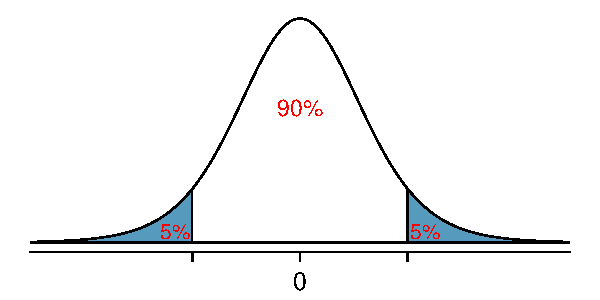
\includegraphics[width=\textwidth]{5-3_diff_two_mean/middle90.pdf}
}}
}

\end{frame}

%%%%%%%%%%%%%%%%%%%%%%%%%%%%%%%%%%%%

\begin{frame}
\frametitle{Valor crítico}
\justifying
\pq{Qual é o $ t ^ \star $ apropriado para um intervalo de confiança para a diferença média entre os preços pontuais de 0,99 e 1 quilate de diamantes?}

\begin{enumerate}[(a)]
\item 1.32
\solnMult{1.72}
\item 2.07
\item 2.82
\end{enumerate}

\only<1>{
{\small
\begin{center}
\begin{tabular}{r | r r r r r}
\hline
uma cauda & \hspace{1.5mm}  0.100 & \hspace{1.5mm} {0.050} & \hspace{1.5mm} {0.025} & \hspace{1.5mm} {0.010} & \hspace{1.5mm} 0.005  \\
duas caudas & 0.200 & 0.100 & 0.050 & 0.020 & 0.010 \\
\hline
df \hfill 21  &  {  1.32} & {  1.72} & {  2.08} & {  2.52} & {  2.83}  \\ 
22  &  {  1.32} & {  1.72} & {  2.07} & {  2.51} & {  2.82}  \\ 
23  &  {  1.32} & {  1.71} & {  2.07} & {  2.50} & {  2.81}  \\ 
24  &  {  1.32} & {  1.71} & {  2.06} & {  2.49} & {  2.80}  \\ 
25  &  {  1.32} & {  1.71} & {  2.06} & {  2.49} & {  2.79}  \\ 
\end{tabular}
\end{center}
}}

\only<2|handout:0>{
\begin{center}
{\small
\begin{tabular}{r | r >{\columncolor[gray]{.6}[.5\tabcolsep]}r r  r r}
\hline
uma cauda & \hspace{1.5mm}  0.100 & \hspace{1.5mm} {0.050} & \hspace{1.5mm} {0.025} & \hspace{1.5mm} {0.010} & \hspace{1.5mm} 0.005  \\
duas caudas & 0.200 & \orange{0.100} & 0.050 & 0.020 & 0.010 \\
\hline
df \hfill 21  &  {  1.32} & {  1.72} & {  2.08} & {  2.52} & {  2.83}  \\ 
  \rowcolor[gray]{.6}
22  &  {  1.32} & \orange{  1.72} & {  2.07} & {  2.51} & {  2.82}  \\ 
23  &  {  1.32} & {  1.71} & {  2.07} & {  2.50} & {  2.81}  \\ 
24  &  {  1.32} & {  1.71} & {  2.06} & {  2.49} & {  2.80}  \\ 
25  &  {  1.32} & {  1.71} & {  2.06} & {  2.49} & {  2.79}  \\ 
\hline
\end{tabular}
}
\end{center}
}


\end{frame}

%%%%%%%%%%%%%%%%%%%%%%%%%%%%%%%%%%%%

\begin{frame}
\frametitle{Intervalo de confiança}
\justifying
\dq{Calcule o intervalo e interprete-o no contexto.}

\pause

\soln{
\[ \text{estimativa pontual} \pm ME \]
\pause
\begin{eqnarray*}
(\bar{x}_{pt99} - \bar{x}_{pt1}) \pm t^\star_{df} \times SE &=& (44.50 - 53.43) \pm 1.72 \times 3.56 \\
\pause
&=& -8.93 \pm  6.12 \\
\pause
&=& (-15.05, -2.81)
\end{eqnarray*}
\pause
\justifying
Temos 90\% de confiança de que o preço médio de um diamante de 0,99 quilates é \$ 15,05 a \$ 2,81 abaixo do preço médio de um diamante de 1 quilate.
}

\end{frame}

%%%%%%%%%%%%%%%%%%%%%%%%%%%%%%%%%%%%

\subsection{Recap}

%%%%%%%%%%%%%%%%%%%%%%%%%%%%%%%%%%%%

\begin{frame}
\frametitle{Recapitulação: Inferência usando diferença de duas médias amostrais pequenas}
\small
\begin{itemize}
\justifying
\item Se $ \sigma_1 $ ou $ \sigma_2 $ for desconhecido, a diferença entre a amostra segue uma distribuição $t$ com $SE = \sqrt{ \frac{s_1^2}{n_1} + \frac{s_2^2}{n_1} }$.

\pause
\justifying
\item Condições: 
\begin{itemize}
\justifying
\item independência dentro dos grupos (frequentemente verificada por uma amostra aleatória, e se amostragem sem reposição, $ n <$ 10 \% da população) e entre grupos.
\justifying
\item nenhum desvio extremo em nenhum dos grupos.
\end{itemize}

\pause
\justifying
\item Teste de hipóteses: 
\[ T_{df} = \frac{\text{estimativa pontual} - \text{valor da hipótese nula}}{SE}\\\text{onde }df = min(n_1 - 1, n_2 - 1) \]

\pause
\justifying
\item Intervalo de confiança:
\[ \text{estimativa pontual} \pm t_{df}^\star \times SE \]

\end{itemize}

\end{frame}

%%%%%%%%%%%%%%%%%%%%%%%%%%%%%%%%%%%


%%%%%%%%%%%%%%%%%%%%%%%%%%%%%%%%%%%%

\section{5.4. Calculando o poder para um teste de 2 amostras}

%%%%%%%%%%%%%%%%%%%%%%%%%%%%%%%%%%%%

\begin{frame}
\frametitle{}

\begin{center}
\begin{tabular}{l l | c c}
\multicolumn{2}{c}{} & \multicolumn{2}{c}{\textbf{Decisão}} \\
& & não rejeitar $H_0$ &  rejeitar $H_0$ \\
  \cline{2-4}
& $H_0$ verdade & \onslide<4->{\green{$1 - \alpha$}} & \onslide<2->{\orange{Erro tipo 1, $\alpha$}} \\
\raisebox{1.5ex}{\textbf{Verdade}} & $H_A$ verdade &  \onslide<3->{\orange{Erro tipo 2, $\beta$}} & \onslide<5->{\green{poder, $1 - \beta$}} \\
  \cline{2-4}
\end{tabular}
\end{center}

\pause

\begin{itemize}
\justifying
\item O erro tipo 1 acontece quando se rejeita $H_0$ quando ela é verdadeira, e a probabilidade de fazer isso é $\alpha$ (nível de significância).

\pause 
\justifying
\item O erro tipo 2 acontece quand se falha em rejeitar $H_0$ ela não é verdadeira, e a probabilidade de fazer isso é $\beta$ (um pouco mais complicado de calcular).

\pause 
\justifying
\item \hl{Poder} de um teste é a probabilidade de rejeitar corretamente $H_0$, e a probabilidade de fazer isso é $ 1 - \beta $.

\pause 
\justifying
\item Nos testes de hipóteses, queremos manter $\alpha$ e $\beta$ baixo, mas existem compensações inerentes.

\end{itemize}

\end{frame}

%%%%%%%%%%%%%%%%%%%%%%%%%%%%%%%%%%%%

\begin{frame}
\frametitle{Taxa de erro tipo 2}
\justifying
Se a hipótese alternativa é realmente verdadeira, qual é a chance de fazermos um Erro Tipo 2, ou seja, deixamos de rejeitar a hipótese nula mesmo quando deveríamos rejeitá-la?

\begin{itemize}
\justifying
\item A resposta não é obvia.
\justifying
\item Se a média real da população estiver muito próxima do valor da hipótese nula, será difícil detectar uma diferença (e rejeitar $ H_0 $).
\justifying
\item Se a média real da população for muito diferente do valor da hipótese nula, será mais fácil detectar uma diferença.
\justifying
\item Claramente, $\beta$ depende do \hl{tamanho do efeito} ($\delta$)
\end{itemize}

\end{frame}

%%%%%%%%%%%%%%%%%%%%%%%%%%%%%%%%%%%%

\begin{frame}
\frametitle{Exemplo - Pressão Arterial (PA), hipóteses}
\justifying
{\dq
{\footnotesize
Suponha que uma empresa farmacêutica tenha desenvolvido uma nova droga para baixar a pressão sanguínea e esteja preparando um ensaio clínico para testar a eficácia da droga. Eles recrutam pessoas que estão tomando uma medicação padrão de pressão sanguínea, e metade dos indivíduos recebe a nova droga (tratamento) e a outra metade continua a tomar a medicação atual com pílulas genéricas para garantir a cegueira (controle). Quais são as hipóteses para um teste de hipóteses bilateral neste contexto?
}
}

\pause

\soln{
\begin{align*}
H_0&: \mu_{tratamento} - \mu_{controle} = 0 \\
H_A&: \mu_{tratamento} - \mu_{controle} \ne 0  
\end{align*}
}

\end{frame}

%%%%%%%%%%%%%%%%%%%%%%%%%%%%%%%%%%%%

\begin{frame}
\frametitle{Exemplo - BP, erro padrão}
\justifying
{\dq
{\footnotesize
Suponha que os pesquisadores gostariam de executar o ensaio clínico em pacientes com pressão arterial sistólica entre 140 e 180 mmHg. Suponha que estudos publicados anteriormente sugiram que o desvio padrão das pressões sanguíneas dos pacientes é de cerca de 12 mmHg e a distribuição das pressões sanguíneas dos pacientes será aproximadamente simétrica. Se tivéssemos 100 pacientes por grupo, qual seria o erro padrão aproximado para diferença nas médias amostrais dos grupos de tratamento e controle?
}
}

\pause

\soln{
\[ SE = \sqrt{ \frac{12^2}{100} + \frac{12^2}{100} } = 1.70 \]
}

\end{frame}

%%%%%%%%%%%%%%%%%%%%%%%%%%%%%%%%%%%%

\begin{frame}
\frametitle{Exemplo - BP, tamanho de efeito mínimo necessário para rejeitar $H_0$}
\justifying
{\dq
{\footnotesize
Para que valores da diferença entre as médias observadas da pressão arterial nos grupos tratamento e controle (tamanho do efeito) rejeitaríamos a hipótese nula no nível de significância de 5\%?}
}

\pause

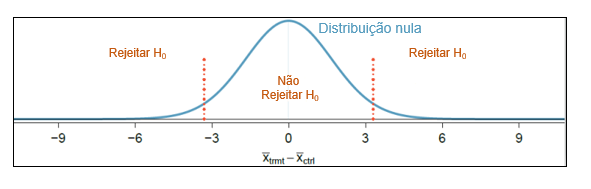
\includegraphics[width=\textwidth]{5-4_power/power_null_B_0_1-7_with_rejection_region.png}

\pause
\small{
\justifying
A diferença deve ser pelo menos 
\[ 1.96 * 1.70 = 3.332 \] 
\justifying
ou no máximo 
\[ -1.96 * 1.70 = 3.332. \]
}
\end{frame}

%%%%%%%%%%%%%%%%%%%%%%%%%%%%%%%%%%%%

\begin{frame}
\frametitle{Exemplo - BP, poder}
\justifying
{\dq
{\footnotesize
Suponha que os pesquisadores da empresa se preocupem em encontrar qualquer efeito na pressão arterial que seja de 3 mmHg ou maior em relação à medicação padrão. Qual é o poder do teste que pode detectar esse efeito?
}}

\pause

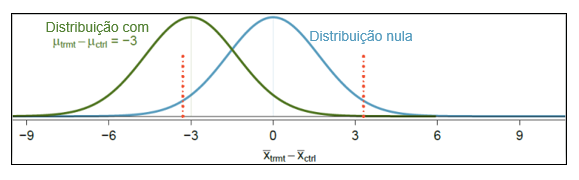
\includegraphics[width=\textwidth]{5-4_power/power_null_C_0_1-7_with_alt_at_3.png}

\pause

\[ Z = \frac{-3.332 - (-3)}{1.70} = -0.20 \]

\pause

\[ P(Z < -0.20) = 0.4207 \]

\end{frame}

%%%%%%%%%%%%%%%%%%%%%%%%%%%%%%%%%%%%

\begin{frame}
\frametitle{Exemplo - BP, tamanho de amostra necessário para 80\% de poder}
\justifying
{\dq
{\footnotesize
Qual tamanho de amostra levará a uma poder de 80\% para este teste?
}}

\pause

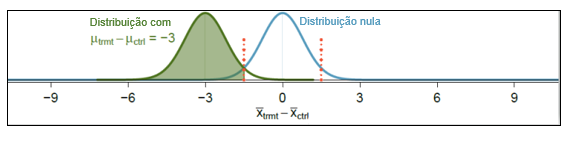
\includegraphics[width=\textwidth]{5-4_power/power_null_0_0-76_with_alt_at_3_and_shaded.png}

\pause
\small{
\[ SE = \frac{3}{2.8} = 1.07142 \]

\pause

\[ 1.07142 = \sqrt{ \frac{12^2}{n} + \frac{12^2}{n} } \]

\pause

\[ n = 250.88 \rightarrow n \ge 251 \]
}
\end{frame}

%%%%%%%%%%%%%%%%%%%%%%%%%%%%%%%%%%%%

\begin{frame}
\frametitle{Recapitulando}

\begin{itemize}
\justifying
\item Calcule o tamanho de amostra necessário para um nível desejado de poder.
\justifying
\item Calcule a poder para uma faixa de tamanhos de amostra e, em seguida, escolha o tamanho da amostra que produz a poder desejado (geralmente 80\% ou 90\%).
\end{itemize}
\begin{center}
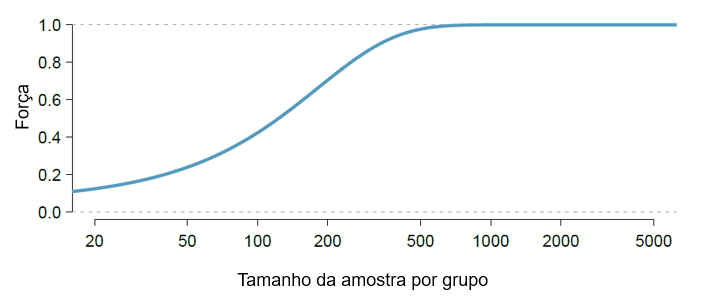
\includegraphics[width=0.7\textwidth]{5-4_power/power_curve_neg-3.png}
\end{center}

\end{frame}

%%%%%%%%%%%%%%%%%%%%%%%%%%%%%%%%%%%%

\begin{frame}
\frametitle{Alcançar o poder desejado}
\justifying
Existem várias maneiras de aumentar o poder (e, portanto, diminuir a taxa de erro do tipo 2):

\pause

\begin{enumerate}
\justifying
\item Aumentar o tamanho da amostra

\pause
\justifying
\item Diminuir o desvio padrão da amostra, que essencialmente tem o mesmo efeito que aumentar o tamanho da amostra (diminuirá o erro padrão). Com um $s$ menor, temos uma chance maior de distinguir o valor nulo da estimativa pontual observada. Isso é difícil de assegurar, mas um processo de medição cauteloso e a limitação da população para que ela seja mais homogênea podem ajudar.

\end{enumerate}
\end{frame}
%%%%%%%%%%%%%%%%%%%%%%%%%%%%%%%%%%%%

\begin{frame}
\frametitle{Alcançar o poder desejado}

\begin{enumerate}[3.]

\justifying
\item Aumente $\alpha$, o que aumentará a probabilidade de rejeitar $H_0$ (mas observe que isso tem o efeito colateral de aumentar a taxa de erro de tipo 1).

\end{enumerate}


\pause
\begin{enumerate}[4.]
\justifying
\item Considere um tamanho de efeito maior. Se a verdadeira média da população estiver na hipótese alternativa, mas próxima do valor nulo, será mais difícil detectar uma diferença.

\end{enumerate}


\end{frame}

%%%%%%%%%%%%%%%%%%%%%%%%%%%%%%%%%%%%


%%%%%%%%%%%%%%%%%%%%%%%%%%%%%%%%%%

\section{5.5. Comparando médias com ANOVA}

%%%%%%%%%%%%%%%%%%%%%%%%%%%%%%%%%%%

\subsection{Aldrin no rio Wolf}

%%%%%%%%%%%%%%%%%%%%%%%%%%%%%%%%%%%

\begin{frame}
\frametitle{Prática}

\begin{center}
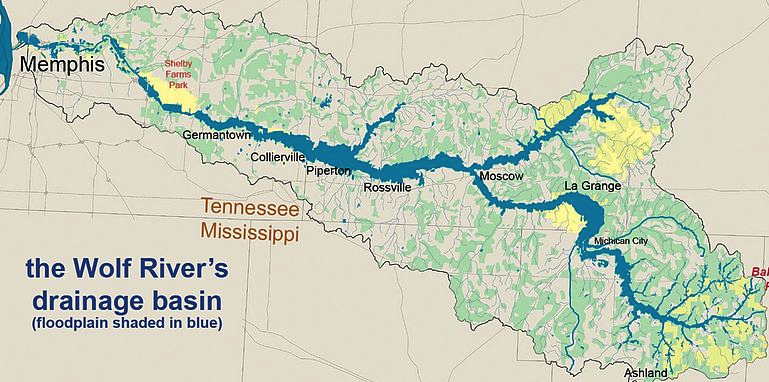
\includegraphics[width=0.7\textwidth]{5-5_anova/wolf.png}
\end{center}

{\small
\begin{itemize}
\justifying
\item O rio Wolf no Tennessee passa por um local abandonado antes utilizado pela indústria de pesticidas para despejar resíduos, incluindo clordano (pesticida), aldrina e dieldrina (ambos inseticidas).

\pause
\justifying
\item Estes compostos orgânicos altamente tóxicos podem causar vários tipos de câncer e problemas congênitos.

\end{itemize}
}
\end{frame}
%%%%%%%%%%%%%%%%%%%%%%%%%%%%%%%%%%%

\begin{frame}
\frametitle{Prática}

{\small
\begin{itemize}
\justifying
\item Os métodos padrão para testar se essas substâncias estão presentes em um rio é coletar amostras a seis décimos de profundidade. 

\pause
\justifying
\item Mas, uma vez que esses compostos são mais densos que a água e suas moléculas tendem a aderir a partículas de sedimento, eles são mais propensos a serem encontrados em concentrações mais altas perto do fundo do que perto da metade da profundidade.

\end{itemize}
}

\end{frame}

%%%%%%%%%%%%%%%%%%%%%%%%%%%%%%%%%%%

\begin{frame}
\frametitle{Dados}
\justifying
Concentração de aldrina (nanogramas por litro) em três níveis de profundidade. \\

\begin{center}
\scalefont{0.7}
\begin{tabular}{r | c | c}
\hline
 	& aldrin 					& depth \\ 
\hline
1 	& \textcolor{darkGray}{3.80} 	& \textcolor{darkGray}{inferior}  \\ 
2 	& \textcolor{darkGray}{4.80} 	& \textcolor{darkGray}{inferior}  \\ 
...	&						& \\
10	& \textcolor{darkGray}{8.80} 	& \textcolor{darkGray}{inferior} \\
11	& \textcolor{blue}{3.20} 		& \textcolor{blue}{meio}  \\
12	& \textcolor{blue}{3.80} 		& \textcolor{blue}{meio} \\
...	&						& \\
20 	& \textcolor{blue}{6.60} 		& \textcolor{blue}{meio} \\
21	& \textcolor{oiB}{3.10} 		& \textcolor{oiB}{superfície} \\
22	& \textcolor{oiB}{3.60} 		& \textcolor{oiB}{superfície} \\
...	&						& \\
30 	& \textcolor{oiB}{5.20} 		& \textcolor{oiB}{superfície} \\  
\hline
\end{tabular}
\end{center}

\end{frame}

%%%%%%%%%%%%%%%%%%%%%%%%%%%%%%%%%%%

\begin{frame}
\frametitle{Análise Exploratória}
\justifying
Concentração de aldrina (nanogramas por litro) em três níveis de profundidade. \\

\begin{center}
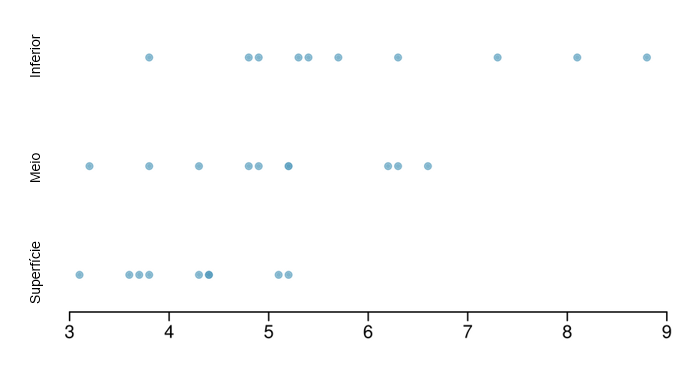
\includegraphics[width=0.65\textwidth]{5-5_anova/dotplot.png}
\end{center}

\begin{center}
\scalefont{0.6}
\begin{tabular}{l | c c c}
		& n	& média	& sd		\\
\hline
inferior	& 10	& 6.04	& 1.58 \\
meio & 10	& 5.05	& 1.10 \\
superficie	& 10	& 4.20	& 0.66 \\
\hline
no geral	& 30	& 5.1	0	& 1.37
\end{tabular}
\end{center}

\end{frame}

%%%%%%%%%%%%%%%%%%%%%%%%%%%%%%%%%%%

\begin{frame}
\frametitle{Questão de pesquisa}
\justifying
\dq{Existe diferença entre as concentrações médias de aldrina entre os três níveis?}

\vspace{0.5cm}

\pause

\begin{itemize}
\justifying
\item Para comparar médias de dois grupos usamos uma estatística Z ou T.

\pause
\justifying
\item Para comparar médias de 3+ grupos, usamos um novo teste chamado \hl{ANOVA} e uma nova estatística chamada \hl{F}.

\end{itemize}

\end{frame}

%%%%%%%%%%%%%%%%%%%%%%%%%%%%%%%%%%%

\begin{frame}
\frametitle{ANOVA}
\justifying
A ANOVA é usada para avaliar se a média da variável é diferente para diferentes níveis de uma variável categórica.

\pause

\begin{itemize}
\justifying
\item[] \mathhl{H_0:} O resultado médio é o mesmo em todas as categorias, 
\[\mu_1 = \mu_2 = \cdots = \mu_k, \]
\justifying
onde $\mu_i$ representa a média do resultado para observações na categoria $i$.
\item[]
\justifying
\item[] \mathhl{H_A:} Pelo menos uma média é diferente das outras.
\end{itemize}

\end{frame}

%%%%%%%%%%%%%%%%%%%%%%%%%%%%%%%%%%%

\begin{frame}
\small
\frametitle{Condições}

\begin{enumerate}
\justifying
\item As observações devem ser independentes dentro e entre os grupos

\begin{itemize}
\justifying
\item Se os dados são provenientes de amostra aleatória simples de menos de 10\% da população, esta condição é satisfeita.
\justifying
\item Verifique com cuidado se os dados podem ser independentes (por exemplo, sem pareamento).
\justifying
\item Sempre importante, mas às vezes difícil de verificar.
\end{itemize}

\pause
\justifying
\item As observações dentro de cada grupo devem ser quase normais.

\begin{itemize}
\justifying
\item Especialmente importante quando os tamanhos das amostras são pequenos.
\end{itemize}
\justifying
\dq{Como podemos verificar a normalidade?}

\pause
\justifying
\item A variabilidade entre os grupos deve ser aproximadamente igual.

\begin{itemize}
\justifying
\item Especialmente importante quando os tamanhos das amostras diferem entre os grupos.
\end{itemize}
\justifying
\dq{Como podemos verificar essa condição?}

\end{enumerate}
\end{frame}


%%%%%%%%%%%%%%%%%%%%%%%%%%%%%%%%%%%

\begin{frame}
\frametitle{$z$/$t$ teste vs. ANOVA - Objetivo}

\twocol{0.5}{0.5}
{\justifying
\[ \hl{$z$/$t$ teste} \]
\justifying
Comparar mpedias de \hl{dois} grupos para ver se elas estão tão distantes que a diferença observada não pode ser atribuída à variabilidade amostral.
\[ H_0: \mu_1 = \mu_2 \]
}
{
\[ \hl{ANOVA} \]
\justifying
Comparar as médias de \hl{dois ou mais} grupos para ver se elas estão tão distantes que as diferenças observadas não podem ser todas atribuídas à variabilidade amostral.
\[ H_0: \mu_1 = \mu_2 = \cdots = \mu_k \]
}

\end{frame}

%%%%%%%%%%%%%%%%%%%%%%%%%%%%%%%%%%%

\begin{frame}
\frametitle{$z$/$t$ teste vs. ANOVA - Método}

\twocol{0.5}{0.5}
{
\[ \hl{$z$/$t$ teste} \]
Calcule uma estatística de teste (uma proporção).
\[ z / t = \frac{(\bar{x}_1 - \bar{x}_2) - (\mu_1 - \mu_2)}{SE(\bar{x}_1 - \bar{x}_2)} \]
}
{
\[ \hl{ANOVA} \]
Calcule uma estatística de teste (uma proporção).
\[ F = \frac{\text{variabilidade entre grupos}}{\text{variabilidade dentro de grupos}} \]
}

\vspace{1cm}

\pause

\begin{itemize}
\justifying
\item Valores grandes das estatísticas de teste levam a valores de p pequenos. 
\justifying
\item Se o valor p for pequeno o suficiente, $H_0$ é rejeitada, concluímos que as médias populacionais não são iguais.

\end{itemize}

\end{frame}

%%%%%%%%%%%%%%%%%%%%%%%%%%%%%%%%%%%

\begin{frame}
\frametitle{$z$/$t$ teste vs. ANOVA}

\begin{itemize}
\justifying
\item Com apenas dois grupos, o teste t e a ANOVA são equivalentes, mas apenas se usarmos uma variância padrão agrupada no denominador da estatística de teste.

\pause
\justifying
\item Com mais de dois grupos, a ANOVA compara as médias amostrais com uma \hl{grande média geral}.

\end{itemize}

\end{frame}

%%%%%%%%%%%%%%%%%%%%%%%%%%%%%%%%%%%

\begin{frame}
\frametitle{Hipóteses}
\justifying
\pq{Quais são as hipóteses corretas para testar a diferença entre as concentrações médias de aldrina entre os três níveis?}

\begin{enumerate}[(a)]
\item $H_0: \mu_B = \mu_M = \mu_S$ \\
$H_A: \mu_B \ne \mu_M \ne \mu_S$ \\
\item $H_0: \mu_B \ne \mu_ M \ne \mu_S$ \\
$H_A: \mu_B = \mu_M = \mu_S$ \\
\solnMult{$H_0: \mu_B = \mu_M = \mu_S$ \\
$H_A:$ Pelo menos uma média é diferente.}
\item $H_0: \mu_B = \mu_M = \mu_S = 0$ \\
$H_A:$ Pelo menos uma média é diferente.
\item $H_0: \mu_B = \mu_M = \mu_S$ \\
$H_A: \mu_B > \mu_M > \mu_S$ \\
\end{enumerate}

\end{frame}

%%%%%%%%%%%%%%%%%%%%%%%%%%%%%%%%%%%

\subsection{ANOVA e o teste F}

%%%%%%%%%%%%%%%%%%%%%%%%%%%%%%%%%%%

\begin{frame}
\frametitle{Estatística de teste}
\justifying
\dq{Parece haver muita variabilidade dentro dos grupos? E que tal entre grupos?}
\justifying
\[ F = \frac{\text{variabilidade entre grupos}}{\text{variabilidade dentro dos grupos}}  \]

\begin{center}
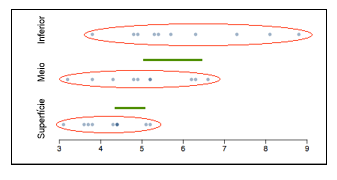
\includegraphics[width=0.75\textwidth]{5-5_anova/dotplot_var.png}
\end{center}

\end{frame}

%%%%%%%%%%%%%%%%%%%%%%%%%%%%%%%%%%%

\begin{frame}
\frametitle{Estatística de teste (cont.)}
\justifying
\[ F = \frac{\text{variabilidade entre grupos}}{\text{variabilidade dentro dos grupos}} = \frac{\hl{MSG}}{\hl{MSE}}  \]

\begin{itemize}
\justifying
\item \hl{MSG} é o quadrado médio entre os grupos
\[ df_G = k - 1 \]
onde $k$ é o número de grupos
\justifying
\item \hl{MSE} é erro quadrático médio - variabilidade dos resíduos
\[ df_E = n - k \]
onde $n$ é o número de observações.

\end{itemize}

\end{frame}
%
%%%%%%%%%%%%%%%%%%%%%%%%%%%%%%%%%%%%

\begin{frame}
\frametitle{$F$ distribuição e valor p}
\justifying
\[ F =  \frac{\text{variabilidade entre grupos}}{\text{variabilidade dentro dos grupos}} \]

\vspace{-1cm}

\begin{center}
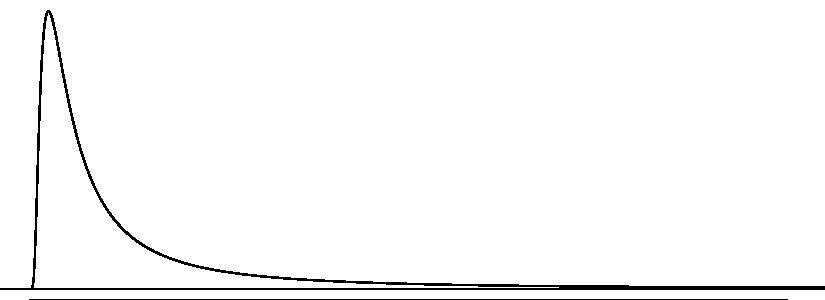
\includegraphics[width=0.75\textwidth]{5-5_anova/fdist.pdf}
\end{center}

\begin{itemize}
\justifying
\item Para podermos rejeitar $ H_0 $, precisamos de um pequeno valor-p, que requer uma estatística F grande.
\justifying
\item Para obter uma estatística F grande, a variabilidade entre as médias da amostra precisa ser maior que a variabilidade dentro das médias amostrais.

\end{itemize}

\end{frame}

%%%%%%%%%%%%%%%%%%%%%%%%%%%%%%%%%%%

\subsection{Saída ANOVA, desconstruída}

%%%%%%%%%%%%%%%%%%%%%%%%%%%%%%%%%%%

\begin{frame}
\frametitle{Graus de liberdade associados à ANOVA}

\vspace{-0.5cm}

{\footnotesize
\begin{center}
\begin{tabular}{ll >{\columncolor[gray]{.6}[.5\tabcolsep]}rrrrr}
\hline
 			& 			& Df 	& Soma Sq	& Média Sq 	& F valor 	& Pr($>$F) \\ 
\hline
(\hl{G}rupo) 	& profundidade 		& 2 	& 16.96 	& 8.48 		& 6.13 	& 0.0063 \\ 
(\hl{E}rro) 	& Resíduos 	& 27 	& 37.33 	& 1.38 		&  		&  \\ 
\hline
	 		& \hl{T}otal	& 29	& 54.29 \\
\end{tabular}
\end{center}
}

\formula{Graus de liberdade associados à ANOVA}
{
\begin{itemize}
\item grupos: $df_G = k - 1$, onde $k$ é o número de grupos
\item total: $df_T = n - 1$, onde $n$ é o tamanho total da amostra
\item erro: $df_E = df_T - df_G$
\end{itemize}
}

\pause

\begin{itemize}

\item $df_G = k - 1 = 3 - 1 = 2$ \\ 

\pause

\item $df_T = n - 1 = 30 - 1 = 29$

\pause

\item $df_E = 29 - 2 = 27$ \\

\end{itemize}

\end{frame}

%%%%%%%%%%%%%%%%%%%%%%%%%%%%%%%%%%%

\begin{frame}
\frametitle{Soma dos quadrados entre os grupos, SSG}

\vspace{-0.25cm}

{\footnotesize
\begin{center}
\begin{tabular}{ll r>{\columncolor[gray]{.6}[.5\tabcolsep]}rrrr}
\hline
 			& 			& Df 	& Soma Sq	& Média Sq 	& F valor 	& Pr($>$F) \\ 
\hline
(\hl{G}rupo) 	& profundidade 		& 2 	& \orange{16.96} 	& 8.48 		& 6.13 	& 0.0063 \\ 
(\hl{E}rro) 	& Resíduos 	& 27 	& 37.33 	& 1.38 		&  		&  \\ 
\hline
	 		& \hl{T}otal	& 29	& 54.29 \\
\end{tabular}
\end{center}
}
\justifying
\formula{Soma dos quadrados entre os grupos, SSG}
{
Mede a variabilidade entre grupos
\vspace{-0.25cm}
\[ SSG = \sum_{i = 1}^{k} n_i (\bar{x}_i - \bar{x})^2 \]
onde $n_i$ é o tamanho de cada grupo, $\bar{x}_i$ é a média para cada grupo, $ \bar {x} $ é a média geral (grande).
}

\end{frame}
%%%%%%%%%%%%%%%%%%%%%%%%%%%%%%%%%%%

\begin{frame}
\frametitle{Soma dos quadrados entre os grupos, SSG}


\vspace{-0.5cm}

\twocol{0.4}{0.5}
{
{\small
\begin{center}
\begin{tabular}{l | c c }
		& n	& média		\\
\hline
inferior	& 10	& 6.04	 \\
meio& 10	& 5.05	 \\
superfície	& 10	& 4.2	 \\
\hline
no geral	& 30	& 5.1	
\end{tabular}
\end{center}
}
}
{
\pause
\begin{eqnarray*}
SSG &=& \pr{ 10 \times (6.04 - 5.1)^2 } \\
\pause
&+& \pr{ 10 \times (5.05 - 5.1)^2 } \\
\pause
&+& \pr{ 10 \times (4.2 - 5.1)^2 } \\
\pause
&=& 16.96 \\
\end{eqnarray*}
}

\end{frame}

%%%%%%%%%%%%%%%%%%%%%%%%%%%%%%%%%%%

\begin{frame}
\frametitle{Soma do total de quadrados SST}

\vspace{-0.25cm}

{\footnotesize
\begin{center}
\begin{tabular}{ll r>{\columncolor[gray]{.6}[.5\tabcolsep]}rrrr}
\hline
 			& 			& Df 	& Soma Sq	& Média Sq 	& F valor 	& Pr($>$F) \\ 
\hline
(\hl{G}rupos) 	& Profundidade 		& 2 	& 16.96	& 8.48 		& 6.13 	& 0.0063 \\ 
(\hl{E}rro) 	& Resíduos 	& 27 	& 37.33 	& 1.38 		&  		&  \\ 
\hline
	 		& \hl{T}otal	& 29	& \orange{54.29} \\
\end{tabular}
\end{center}
}
\justifying
\formula{Soma do total de quadrados SST}
{
Mede a variabilidade entre grupos 
\vspace{-0.25cm}
\[ SST = \sum_{i = 1}^{n} (x_i - \bar{x}) \]
onde $x_i$ representam cada observação no conjunto de dados.
}

\pause

\vspace{-0.75cm}

\begin{eqnarray*}
SST &=& (3.8 - 5.1)^2 + (4.8 - 5.1)^2 + (4.9 - 5.1)^2 + \cdots + (5.2 - 5.1)^2 \\
\pause
&=& (-1.3)^2 + (-0.3)^2 + (-0.2)^2 + \cdots + (0.1)^2 \\
\pause
&=& 1.69 + 0.09 + 0.04 + \cdots + 0.01 \\
\pause
&=& 54.29
\end{eqnarray*}

\end{frame}

%%%%%%%%%%%%%%%%%%%%%%%%%%%%%%%%%%%

\begin{frame}
\frametitle{Soma dos quadrados erro, SSE}

\vspace{-0.25cm}

{\footnotesize
\begin{center}
\begin{tabular}{ll r>{\columncolor[gray]{.6}[.5\tabcolsep]}rrrr}
\hline
 			& 			& Df 	& Soma Sq	& Média Sq 	& F valor 	& Pr($>$F) \\ 
\hline
(\hl{G}rupo) 	& Profundidade 		& 2 	& 16.96	& 8.48 		& 6.13 	& 0.0063 \\ 
(\hl{E}rro) 	& Resíduos 	& 27 	& \orange{37.33} 	& 1.38 		&  		&  \\ 
\hline
	 		& \hl{T}otal	& 29	& 54.29 \\
\end{tabular}
\end{center}
}

\formula{Soma dos quadrados erro, SSE}
{
Mede a variabilidade dentro de grupos:
\[ SSE = SST - SSG \]
}

\pause

\[ SSE =  54.29 - 16.96 =  37.33 \]

\end{frame}

%%%%%%%%%%%%%%%%%%%%%%%%%%%%%%%%%%%

\begin{frame}
\frametitle{Erro quadrático médio}

\vspace{-0.25cm}

{\footnotesize
\begin{center}
\begin{tabular}{ll rr>{\columncolor[gray]{.6}[.5\tabcolsep]}rrr}
\hline
 			& 			& Df 	& Soma Sq	& Média Sq 	& F valor 	& Pr($>$F) \\ 
\hline
(\hl{G}rupo) 	& profundidade 		& 2 	& 16.96	& \orange{8.48} 		& 6.13 	& 0.0063 \\ 
(\hl{E}rro) 	& Resíduos 	& 27 	& 37.33 	& \orange{1.38} 		&  		&  \\ 
\hline
	 		& \hl{T}otal	& 29	& 54.29 \\
\end{tabular}
\end{center}
}
\justifying
\formula{Erro quadrático médio}
{
O erro quadrático médio é calculado como a soma dos quadrados divididos pelos graus de liberdade.
}

\pause

\begin{eqnarray*}
MSG &=& 16.96 / 2 = 8.48 \\
\pause
MSE &=& 37.33 / 27 = 1.38
\end{eqnarray*}

\end{frame}

%%%%%%%%%%%%%%%%%%%%%%%%%%%%%%%%%%%

\begin{frame}
\frametitle{Estatística de teste, valor F}

\vspace{-0.25cm}

{\footnotesize
\begin{center}
\begin{tabular}{ll rrr>{\columncolor[gray]{.6}[.5\tabcolsep]}rr}
\hline
 			& 			& Df 	& Soma Sq	& Média Sq 	& F valor 	& Pr($>$F) \\ 
\hline
(\hl{G}rupo) 	& Profundidade 		& 2 	& 16.96	& 8.48 		& \orange{6.14} 	& 0.0063 \\ 
(\hl{E}rro) 	& Resíduos 	& 27 	& 37.33 	& 1.38 		&  		&  \\ 
\hline
	 		& \hl{T}otal	& 29	& 54.29 \\
\end{tabular}
\end{center}
}
\justifying
\formula{Estatística de teste, valor F}
{
Como discutimos anteriormente, a estatística F é a razão entre o grupo e a variabilidade dentro do grupo.
\[ F = \frac{MSG}{MSE} \]
}

\pause

\[ F = \frac{8.48}{1.38} = 6.14 \]

\end{frame}

%%%%%%%%%%%%%%%%%%%%%%%%%%%%%%%%%%%

\begin{frame}
\frametitle{valor-p}

\vspace{-0.25cm}

{\footnotesize
\begin{center}
\begin{tabular}{ll rrr>{\columncolor[gray]{.6}[.5\tabcolsep]}rr}
\hline
 			& 			& Df 	& Soma Sq	& Média Sq 	& F valor 	& Pr($>$F) \\ 
\hline
(\hl{G}rupo) 	& profundidade 		& 2 	& 16.96	& 8.48 		& \orange{6.14} 	& 0.0063 \\ 
(\hl{E}rro) 	& Resíduos 	& 27 	& 37.33 	& 1.38 		&  		&  \\ 
\hline
	 		& \hl{T}otal	& 29	& 54.29 \\
\end{tabular}
\end{center}
}
\justifying
\formula{valor-p}
{
O valor-p é a probabilidade de pelo menos uma relação tão grande entre a variabilidade "entre grupo" e "dentro do grupo", se de fato os meios de todos os grupos são iguais. É calculado como a área sob a curva F, com graus de liberdade $df_G$ e $df_E$, acima da estatística F observada.
}

\pause

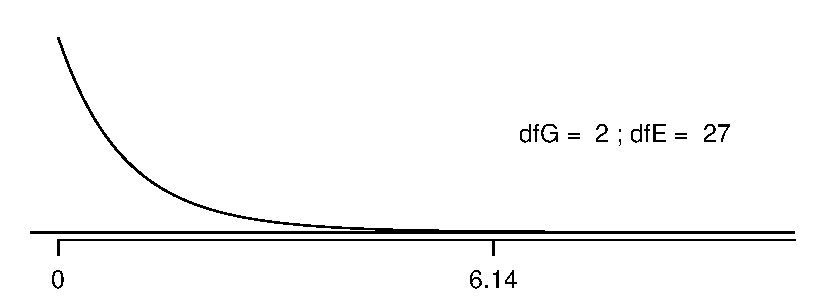
\includegraphics[width=0.5\textwidth]{5-5_anova/f.pdf}

\end{frame}

%%%%%%%%%%%%%%%%%%%%%%%%%%%%%%%%%%%

\begin{frame}
\frametitle{Conclusão - no contexto}
\justifying
\pq{Qual é a conclusão do teste de hipóteses?}

$\:$ \\
\justifying
Os dados fornecem evidências de que a concentração média de aldrina
\begin{enumerate}[(a)]
\justifying
\item  é diferente para todos os grupos.
\justifying
\item na superfície é menor que os outros níveis.
\justifying
\solnMult{é diferente para pelo menos um grupo.}
\justifying
\item é o mesmo para todos os grupos.

\end{enumerate}

\end{frame}

%%%%%%%%%%%%%%%%%%%%%%%%%%%%%%%%%%%

\begin{frame}
\frametitle{Conclusão}

\begin{itemize}
\justifying
\item  Se valor-p for pequeno (menor que $\alpha$), rejeite $H_0$. Os dados fornecem evidências de que pelo menos uma média é diferente (mas não podemos dizer qual).

\pause
\justifying
\item Se o valor p for grande, não rejeite $H_0$. Os dados não fornecem evidências de que pelo menos um par de médias são diferentes umas das outras, as diferenças observadas nas médias amostrais são atribuíveis à variabilidade amostral (ou acaso).

\end{itemize}

\end{frame}

%%%%%%%%%%%%%%%%%%%%%%%%%%%%%%%%%%%

\subsection{Condições de verificação}

%%%%%%%%%%%%%%%%%%%%%%%%%%%%%%%%%%%

\begin{frame}[fragile]
\frametitle{(1) Independência}
\justifying
\dq{Esta condição parece estar satisfeita?}
\justifying
\soln{\only<2>{Neste estudo, não temos razão para acreditar que a concentração de Aldrin não seja independente uma da outra...}}

\end{frame}

%%%%%%%%%%%%%%%%%%%%%%%%%%%%%%%%%%%

\begin{frame}[fragile]
\frametitle{(2) Aproximadamente normal}
\justifying
\dq{Esta condição parece estar satisfeita?}

\begin{center}
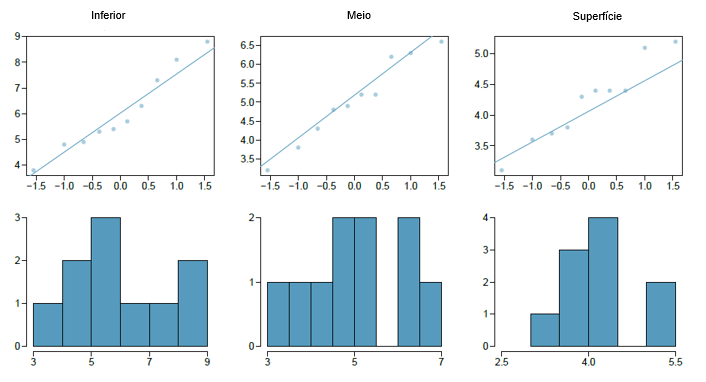
\includegraphics[width=\textwidth]{5-5_anova/normal.png}
\end{center}

\end{frame}

%%%%%%%%%%%%%%%%%%%%%%%%%%%%%%%%%%%

\begin{frame}[fragile]
\frametitle{(3) Variância constante}
\justifying
\dq{Esta condição parece estar satisfeita?}

\begin{center}
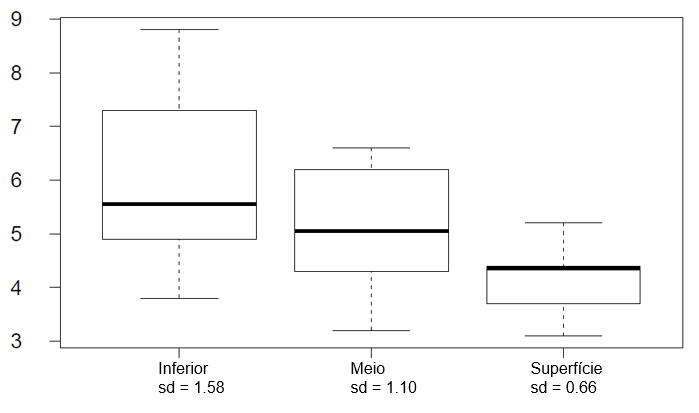
\includegraphics[width=0.7\textwidth]{5-5_anova/homo.png}
\end{center}

\end{frame}

%%%%%%%%%%%%%%%%%%%%%%%%%%%%%%%%%%%

\subsection{Múltiplas comparações \& taxa de erro tipo 1}

%%%%%%%%%%%%%%%%%%%%%%%%%%%%%%%%%%%

\begin{frame}
\frametitle{O que significa diferir?}

\begin{itemize}
\justifying
\item Anteriormente, concluímos que pelo menos um par de médias diferem. A questão natural que se segue é "quais?"

\pause
\justifying
\item Podemos fazer dois testes $ t $ de amostra para diferenças em cada par de grupos possível.

\pause

\end{itemize}
\justifying
\dq{Você consegue ver alguma armadilha com essa abordagem?}

\pause

\begin{itemize}
\justifying
\item Quando executamos muitos testes, a taxa de erro do tipo 1 aumenta.
\justifying
\item Esse problema é resolvido usando um nível de significância modificado.

\end{itemize}

\end{frame}

%%%%%%%%%%%%%%%%%%%%%%%%%%%%%%%%%%%

\begin{frame}
\frametitle{Comparações Múltiplas}

\begin{itemize}
\justifying
\item O cenário de testar muitos pares de grupos é chamado \hl{comparações múltiplas}.

\pause
\justifying
\item A \hl{correção de Bonferroni} sugere que um nível de significância mais \orange{rigoroso} é mais apropriado para estes testes:

\[ \alpha^\star = \alpha / K \]
\justifying
onde $K$ é o número de comparações consideradas.

\pause
\justifying
\item Se existem grupos $k$, então todos os pares possíveis são comparados e $K = \frac{k (k - 1)}{2}$.

\end{itemize}

\end{frame}

%%%%%%%%%%%%%%%%%%%%%%%%%%%%%%%%%%%

\begin{frame}
\frametitle{Determinando o modificado $\alpha$}
\justifying
\pq{No aldrin, a profundidade do conjunto de dados tem 3 níveis: inferior, média e superfície. Se $\alpha = 0.05$, qual deve ser o nível de significância modificado para dois testes $t$ de amostra para determinar quais pares de grupos possuem médias significativamente diferentes?}

\begin{enumerate}[(a)]
\item $\alpha^* = 0.05$
\item $\alpha^* = 0.05 / 2 = 0.025$
\solnMult{$\alpha^* = 0.05 / 3 = 0.0167$}
\item $\alpha^* = 0.05 / 6 = 0.0083$
\end{enumerate}

\end{frame}

%%%%%%%%%%%%%%%%%%%%%%%%%%%%%%%%%%%

\begin{frame}
\frametitle{O que significa diferir?}
\justifying
\pq{Com base nos gráficos abaixo, o que significa que você esperaria ser significativamente diferente?}

\twocol{0.6}{0.4}{
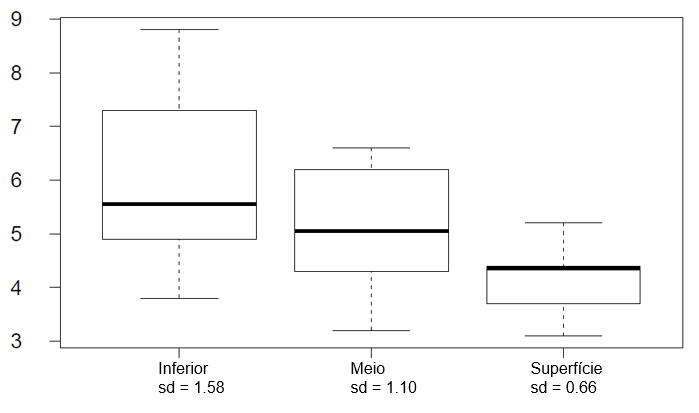
\includegraphics[width=\textwidth]{5-5_anova/homo.png}
}
{
\begin{enumerate}[(a)]
\item inferior \& superfície
\item inferior \& meio
\item meio \& superfície
\item inferior \& meio; meio \& superfície
\item inferior \& meio; inferior \& superfície; meio \& superfície
\end{enumerate}
}

\end{frame}

%%%%%%%%%%%%%%%%%%%%%%%%%%%%%%%%%%

\begin{frame}
\frametitle{O que significa diferir? (cont.)}
\justifying
Se a suposição de variabilidade igual entre os grupos for satisfeita para a ANOVA, podemos usar os dados de todos os grupos para estimar a variabilidade:
 
\begin{itemize}
\justifying
\item Estime qualquer desvio padrão dentro do grupo com $ \sqrt {MSE} $, que é $s_{agrupado}$
\justifying
\item Use os graus de liberdade do erro, $n - k$, para a distribuição $t$.

\end{itemize}
\justifying
\formula{Diferença entre duas médias: após ANOVA}{
\[ SE = \sqrt{  \frac{\sigma_1^2}{n_1} + \frac{\sigma_2^2}{n_2} } \approx \sqrt{ \frac{MSE}{n_1} + \frac{MSE}{n_2} } \]
}

\end{frame}

%%%%%%%%%%%%%%%%%%%%%%%%%%%%%%%%%%

\begin{frame}
\frametitle{Prática}
\justifying
\dq{Existe uma diferença entre a concentração média de aldrina na parte inferior e a meia profundidade?}

\twocol{0.4}{0.7}{
{\scriptsize
\begin{center}
\scalefont{0.8}
\begin{tabular}{l | c c c}
		& n	& média	& sd		\\
\hline
inferior	& 10	& \orange{6.04}	& 1.58 \\
meio& 10	& \orange{5.05}	& 1.10 \\
superfície	& 10	& 4.2 	& 0.66 \\
\hline
no geral	& 30	& 5.1		& 1.37
\end{tabular}
\end{center}
}
}
{
{\scriptsize
\begin{center}
\scalefont{0.8}
\begin{tabular}{l rrrrr}
\hline
 			& Df 	& Soma Sq	& Média Sq 	& F valor 	& Pr($>$F) \\ 
\hline
profundidade 		& 2 	& 16.96 	& 8.48 		& 6.13 	& 0.0063 \\ 
Resíduos 	& \orange{27} 	& 37.33 	& \orange{1.38} 		&  		&  \\ 
\hline
Total			& 29	& 54.29 \\
\end{tabular}
\end{center}
}
}
\scalefont{0.7}
\begin{eqnarray*}
T_{df_E} &=& \frac{(\bar{x}_{inferior} - \bar{x}_{meio})}{\sqrt{ \frac{MSE}{n_{inferior}} + \frac{MSE}{n_{meio}} }} \\ 
\pause
T_{27} &=& \frac{( 6.04 - 5.05 )}{\sqrt{ \frac{1.38}{10} + \frac{1.38}{10} }} = \frac{0.99}{0.53}  =1.87 \\
\pause
0.05 &<& valor-p < 0.10 \qquad \text{{\footnotesize (frente e verso)}} \\
\pause
\alpha^\star &=& 0.05 / 3 = 0.0167
\end{eqnarray*}
\justifying
\pause
{\small Não rejeite $H_0$, os dados não fornecem evidências convincentes de uma diferença entre as concentrações médias de aldrina na profundidade inferior e média.}

\end{frame}

%%%%%%%%%%%%%%%%%%%%%%%%%%%%%%%%%%

\begin{frame}
\frametitle{Prática}
\justifying
\app{Comparações entre pares} {Existe uma diferença entre a concentração média de aldrina no fundo e na superfície?}

\pause

\soln{
\begin{eqnarray*}
T_{df_E} &=& \frac{(\bar{x}_{inferior} - \bar{x}_{superfície})}{\sqrt{ \frac{MSE}{n_{inferior}} + \frac{MSE}{n_{superficie}} }} \\ 
\pause
T_{27} &=& \frac{( 6.04 - 4.02 )}{\sqrt{ \frac{1.38}{10} + \frac{1.38}{10} }} = \frac{2.02}{0.53}  =3.81 \\
\pause
valor-p &<& 0.01 \qquad \text{{\footnotesize (frente e verso)}} \\
\pause
\alpha^\star &=& 0.05 / 3 = 0.0167
\end{eqnarray*}
\pause
\justifying
{\small Rejeite $H_0$, os dados fornecem evidências convincentes de uma diferença entre as concentrações médias de aldrina no fundo e na superfície.}
}

\end{frame}

%%%%%%%%%%%%%%%%%%%%%%%%%%%%%%%%%%




%%%%%%%%%%%%%%%%%%%%%%%%%%%%%%%%%%%%
% End document
%%%%%%%%%%%%%%%%%%%%%%%%%%%%%%%%%%%%

\end{document}